% mnras_template.tex 
%
% LaTeX template for creating an MNRAS paper
%
% v3.0 released 14 May 2015
% (version numbers match those of mnras.cls)

%%%%%%%%%%%%%%%%%%%%%%%%%%%%%%%%%%%%%%%%%%%%%%%%%%
% Basic setup. Most papers should leave these options alone.
\documentclass[fleqn,usenatbib]{mnras}

% MNRAS is set in Times font. If you don't have this installed (most LaTeX
% installations will be fine) or prefer the old Computer Modern fonts, comment
% out the following line
\usepackage{newtxtext,newtxmath}
% Depending on your LaTeX fonts installation, you might get better results with one of these:
\usepackage{amsmath}
%\usepackage{mathptmx}
%\usepackage{txfonts}
% Use vector fonts, so it zooms properly in on-screen viewing software
% Don't change these lines unless you know what you are doing
\usepackage[T1]{fontenc}

% Allow "Thomas van Noord" and "Simon de Laguarde" and alike to be sorted by "N" and "L" etc. in the bibliography.
% Write the name in the bibliography as "\VAN{Noord}{Van}{van} Noord, Thomas"
\DeclareRobustCommand{\VAN}[3]{#2}
\let\VANthebibliography\thebibliography
\def\thebibliography{\DeclareRobustCommand{\VAN}[3]{##3}\VANthebibliography}


%%%%% AUTHORS - PLACE YOUR OWN PACKAGES HERE %%%%%

% Only include extra packages if you really need them. Common packages are:
\usepackage{graphicx}	% Including figure files
\usepackage{amsmath}	% Advanced maths commands
%\usepackage{amssymb}	% Extra maths symbols

%%%%%%%%%%%%%%%%%%%%%%%%%%%%%%%%%%%%%%%%%%%%%%%%%%

%%%%% AUTHORS - PLACE YOUR OWN COMMANDS HERE %%%%%

% Please keep new commands to a minimum, and use \newcommand not \def to avoid
% overwriting existing commands. Example:
%\newcommand{\pcm}{\,cm$^{-2}$}	% per cm-squared

%%%%%%%%%%%%%%%%%%%%%%%%%%%%%%%%%%%%%%%%%%%%%%%%%%

%%%%%%%%%%%%%%%%%%% TITLE PAGE %%%%%%%%%%%%%%%%%%%

% Title of the paper, and the short title which is used in the headers.
% Keep the title short and informative.
\title[Modelling stars with GP]{Modelling stars with Gaussian Process Regression -- I:  Augmenting Stellar Model Grid}

% The list of authors, and the short list which is used in the headers.
% If you need two or more lines of authors, add an extra line using \newauthor
\author[T. Li et al.]{
Tanda Li,$^{1}$\thanks{E-mail: t.li.2@bham.ac.uk}
Guy R. Davies,$^{1}$\thanks{E-mail: G.R.Davies@bham.ac.uk}
Alex Lyttle,$^{1}$
Lindsey Carboneau,$^{1}$
and A. N. Others$^{1}$
\\
% List of institutions
$^{1}$ School of Physics and Astronomy, University of Birmingham, Birmingham, B15 2TT, United Kingdom\\
}

% These dates will be filled out by the publisher
\date{Accepted XXX. Received YYY; in original form ZZZ}

% Enter the current year, for the copyright statements etc.
\pubyear{2020}

% Don't change these lines
\begin{document}
\label{firstpage}
\pagerange{\pageref{firstpage}--\pageref{lastpage}}
\maketitle

% Abstract of the paper
\begin{abstract}
Grid-based modelling is widely used for estimating stellar parameters. However, stellar model grid is sparse because of the computational cost. This paper demonstrates an application of Gaussian Process (GP) Regression that turns a sparse model grid to a continuous function. We train GP models to map five fundamental inputs (mass, equivalent evolutionary phase, initial metallicity, initial helium fraction, and the mixing-length parameter) to observable outputs (effective temperature, surface gravity, radius, surface metallicity, and stellar age). 
%
We preliminarily test different approaches with a small subset of data and set up the training with the most promising methods. To overcome the limitation of training data size in the GP framework, we section the whole grid and train each section separately. 
%
An off-grid stellar model dataset is then used to test GP predictions. We find no obvious systematic offsets for all five outputs. The median testing error is $\sim$2K for effective temperature, $\sim 0.001$dex for surface gravity, $\sim$ 0.002$\rm R_{\odot}$ for radius, $\sim 0.001$dex for surface metallicity, and $\sim$0.02Gyr for stellar age. However, we find that local systematic uncertainty is not uniform across the parameter space and it mainly varies with mass, equivalent evolutionary phase, and initial metallicity. We hence train another GP model to describe the systematic uncertainties.      
%
We lastly use 100 fake stars to validate the accuracy of GP for modelling stars. GP-determined masses and ages are well consistent with true values within one standard deviation. We also note that GP models give sensible statistical sampling which overcomes the under-sampling issue in the grid-based modelling. 
%
\end{abstract}

% Select between one and six entries from the list of approved keywords.
% Don't make up new ones.
\begin{keywords}
Star: Modelling -- Machine Learning -- keywords
\end{keywords}

%%%%%%%%%%%%%%%%%%%%%%%%%%%%%%%%%%%%%%%%%%%%%%%%%%

%%%%%%%%%%%%%%%%% BODY OF PAPER %%%%%%%%%%%%%%%%%%
%\section{Outline}
This is a temporary section for the outline/to-do list. 
\begin{itemize}
\item[•] Framework of GP: model data augmentation with the established model grid
\item[•] Two strategies: S1 is from observables to fundamentals for modelling stars; S2 is from fundamentals to observables for augmenting model grids. \item[•] Step 1: selection of GP model inputs. Key points include independence of inputs and overlapping of the ranges of base data. 
\item[•] Step 2: selection of GP kernels and validation. 
\item[•] Step 3: uncertainty analysis. Key points include unreliable GP variance and the produce of uncertainty estimating.
\item[•] Step 4: Application of S1: 1) fake stars (MS, turn-off, subgiant) 2) real stars (the Sun, turn-off star, subgiant star) 3) solar calibration
\item[•] Step 5: Application of S2: augmenting the base grid (challenges, limitations due to grid step etc.)
\end{itemize} 


\section{Introduction}

This will be the intro. (ask Guy to write some general idea of Gaussian Process and the GPR model).

% Set the context of the work.
% Cite relevant earlier studies

%% Lots of work on estimating stellar properties where observables are compared with stellar models.  Typical approach is grid based.  Lots of citations.  

%% Observables can come from all over.  Spectroscopic surveys (APOGEE, Galah, LAMOST, Gaia ESO, +), Astrometric Gaia, Photometric variability CoRoT, Kepler, K2, TESS, soon PLATO.

%% Lots of different models available with lots of different flavours - ask Tanda ...

%% Typical parameters to vary can refer to the star (mass, age, [Fe/H], Y_i) or they can refer to the model (MLT, overshoot, diffusion).  Most studies, certainly for field stars, treat all parameters as being independent.  

% Describe the problem we aim to solve

%% Plenty of work exists on HBM models in astro (cite fest).  By pooling together parameters we can win - for example EB's/cluster age, chemical comp.  But also we could pool parameters of the models MLT, Ov.  If we take a Bayesian approach the pooled constraint on MLT or Ov has the ability to constrain stellar parameters (e.g., age, mass).  The posterior distribution is a joint distribution!

%% Curent limitation is that this is all very tricky computationally.  Great news though - breakthroughs in machine learning, sampling methods, and GPU implementation means we now have a shot at doing this.  In this paper we give a deminstration of principle for one way of proceeding.

% Layout of this paper ...

%% In this paper we describe the computation of a representitative, but not ideal, grid for the purpose of estimating stellar parameters.  We then teach a NN to learn this grid, to act a function approximator.  We then implement the NN in a hierarchical model leveraging the NN backpropagation that allows use to use a gradient based NUTS sampling technique.  We demostrate the methods ability to recover stellar properties and model properties for a set of stars taken from the grid of models used.  Finally we discuss the limitations of this approach and highlight areas where improvements can be found in the near future.


\section{Theoretical  model grid}\label{sec:grid}

We built up a model grid as the training data for GPR models.  We aimed to cover stars with approximate solar mass on the main-sequence and the subgiant phases. Thus, the mass range is set up as 0.8 -- 1.2$M_{\odot}$, and we computed each stellar evolutionary track from the Hayashi line and terminated at the base of red-giant branch where $\log g$ = 3.6 dex. The gird includes four independent model inputs: stellar mass (M), initial helium fraction ($Y_{\rm init}$), initial metallicity ([Fe/H]), and the mixing-length parameter ($\alpha_{\rm MLT}$). Details of the computations are summarised in Table \ref{tab:grid}. Input parameters of our primary training data is uniformly spaced except the input metallicity, which is double dense above 0.2 $dex$. We also computed an extra grid that fit in between the primary training data for $M > 1.05M_{\odot}$. Because evolutionary tracks in this mass range have the so-called 'hook' at the late main-sequence stage and relatively difficult to model. Lastly, we computed 4,880 tracks with input parameters that are randomly sampled in the grid ranges for validating GPR models. The evolution time step was mainly controlled by the set-up tolerances on changes in surface effective temperature and luminosity. We also saved structural models for computing theoretical oscillation models.

\begin{table*}
	\centering
	\caption{Stellar model computations for training and validating sets.}
	\label{tab:grid}
	\begin{tabular}{llll} % four columns, alignment for each
		\hline
		\multicolumn{4}{c}{Primary Grid}\\
		\hline
		Input Parameter & Range & Increment \\
        \hline
	$M$ [$M_{\odot}$]  & 0.80 -- 1.20 &  0.01&\\
        $\rm{[Fe/H]}$ [dex] & -0.5 -- 0.2/0.2 -- 0.5 & 0.1/0.05\\
        	$Y_{\rm init}$ & 0.24 -- 0.32 & 0.02&\\
        $\alpha_{\rm{MLT}}$  & 1.7 -- 2.5&  0.2&\\
        \hline
       \multicolumn{4}{c}{Extra Grid}\\
	\hline
	Input Parameter & Range & Increment \\
        \hline
	$M$ [$M_{\odot}$]  & 1.055 -- 1.195 &  0.01&\\
        $\rm{[Fe/H]}$ [dex] & 0.25 -- 0.45 & 0.1\\
        	$Y_{\rm init}$ & 0.25 -- 0.31 & 0.02&\\
        $\alpha_{\rm{MLT}}$  & 1.8-- 2.4&  0.2&\\
        %Other physics & \multicolumn{2}{Scheme}\\
        %\hline
        %Diffusion & \multicolumn{2}{Yes}\\
        %Overshooting & \multicolumn{2}{N/A}\\
        \hline
        \multicolumn{4}{c}{Off-grid Models}\\
        \hline
        \multicolumn{4}{c}{4880 tracks with random input parameters }\\
	\hline
	\end{tabular}
\end{table*}

\subsection{Stellar models and input physics}\label{subsec:stellar_model}

We used Modules for Experiments in Stellar Astrophysics
(\textsc{MESA}, version 12115) to establish a grid of stellar models. 
\textsc{MESA} is an open-source stellar evolution package which is undergoing active development. Descriptions of input physics and numerical methods
can be found in \citet{2011ApJS..192....3P,2013ApJS..208....4P, 2015ApJS..220...15P}.
We adopted the solar chemical mixture [$(Z/X)_{\odot}$ = 0.0181]
provided by \citet{2009ARA&A..47..481A}. 
The initial chemical composition was calculated by: 
\begin{equation}
\log (Z_{\rm{init}}/X_{\rm{init}}) = \log (Z/X)_{\odot} + \rm{[Fe/H]}.  \\
\end{equation}
We used the \textsc{MESA} $\rho-T$ tables based on the 2005
update of OPAL EOS tables \citep{2002ApJ...576.1064R} and OPAL opacity
supplemented by low-temperature opacity \citep{2005ApJ...623..585F}. 
The MESA ‘simple’ photosphere were used as the set of boundary conditions for modelling the atmosphere.
The mixing-length theory of convection was implemented, where 
$\alpha_{\rm MLT} = \ell_{\rm MLT}/H_p$ is the mixing-length parameter.
We also applied the \textsc{MESA} predictive mixing scheme \citep{2018ApJS..234...34P,2019ApJS..243...10P}  in the model computation. The \textsc{MESA} inlist used for the computation is available on \url{https://github.com/litanda/mesa_inlist}.  

\subsection{Oscillation models and seismic $\Delta \nu$}\label{subsec:seismo_model}

Theoretical stellar oscillations were calculated with the \textsc{GYRE} code (version 5.1), which was developed by \citet{2013MNRAS.435.3406T}. And we computed radial modes (for $\ell$ = 0) by solving the adiabatic stellar pulsation equations with the structural models generated by \textsc{MESA}. We computed a seismic large separation($\Delta \nu$) for each model with theoretical radial modes to avoid the systematic offset of the scaling relation. We derived $\Delta \nu$ with the approach given by \citet{2011ApJ...743..161W}, which is a weighted least-squares fit to the radial frequencies as a function of $n$.  




\section{Gaussian Process regression}\label{GPR}

We adopted the GPy package \citep{gpy2014}, which is a Gaussian Process (GP) framework developed by the Sheffield machine learning group, to train GP models for the \textsc{MESA} Grid. 

\subsection{Gaussian process model}

GP models can be applied as probabilistic models to regression problems.  Here we will use the GP model to generalise a grid of stellar models to a continuous and probabilistic function that maps inputs (i.e., initial mass, composition, age, ...) to observable quantities (i.e., effective temperature, radius, $\Delta \nu$, ... ).  We aim to use the GP model as a non-parametric emulator, that is emulating the comparatively slow calls to models of stellar evolution. 

\subsubsection{Gaussian process application}

We start with a grid of stellar models containing $N$ models with a label we  want to learn, for example model effective temperature, which we will denote with the general symbol $\bf y$, and a set of input labels $\bf X$ (e.g., mass, age, and metallicity).  We can use a GP to make predictions of the effective temperature (or $y$) for additional input values given by $\bf X_{\star}$.  The vector $\bf y$ is arranged ${\bf y} = \left(y_{i}, ... ,y_{N} \right)^{T}$ where the subscript label references the stellar model.  The input labels are arranged into a $N \times D$ matrix where $D$ is the number of input dimensions (e.g., $D=3$ for mass, age, and metallicity) so that ${\bf X} = ({\bf x}_{1}, ..., {\bf x}_{N})^{T}$ where ${\bf x_{i}} = (x_{1, i}, ..., x_{D, i})^{T}$.  The matrix of additional inputs $\bf X_{\star}$ has the same form as $\bf X$ but size $N_{\star} \times D$.

Rasmussen and Williams (!REF!), from which our description below is based, define a GP as a collection of random variables, where any finite number of which have a joint Gaussian distribution.  In general terms, GP's may be written as
\begin{equation}
y({\bf x}) \sim \mathcal{GP}\left( m({\bf x}), {\bf \Sigma}\right),
\end{equation}
where $m({\bf x})$ is some mean function, and ${\bf \Sigma}$ is some covariance matrix.  The mean function controls the deterministic part of the regression and the covariance controls the stochastic part.  The mean function defined here could be any deterministic function and we will label the additional parameters, or hyperparameters, $\phi$.  Each element of the covariance matrix is defined by the covariance function or {\it kernel function} $k$ which has hyperparameters $\theta$ and is given by,
\begin{equation}
{\bf \Sigma}_{n, m} = k({\bf x}_{n}, {\bf x}_{m}),
\end{equation}
where the inputs ${\bf x}_{i}$ are $D$-dimensional vectors and the output is a scalar covariance.

As a GP is a collection of random variables, where any finite number of which have a joint Gaussian distribution, the joint probability of our data $\bf y$ is
\begin{equation}
p({\bf y} | {\bf X, \phi, \theta}) = \mathcal{N}(m({\bf X}), {\bf \Sigma}).
\end{equation}
If we want to obtain predictive distributions for the output $\bf y_{\star}$ given the inputs $\bf X_{\star}$ the joint probability distribution of $\bf y$ and $\bf y_{\star}$ is Gaussian and given by
\begin{equation}
p \left( \begin{bmatrix} {\bf y} \\ {\bf y_{\star}} \end{bmatrix} \right) = \mathcal{N} \left( \begin{bmatrix} {\bf X} \\ {\bf X_{\star}} \end{bmatrix} , \begin{bmatrix} {\bf \Sigma} & {\bf K_{\star} }\\ {\bf K_{\star}}^{T} & {\bf K_{\star \star}} \end{bmatrix}  \right), 
\end{equation}
where the covariance matrices $\bf \Sigma$ and $\bf K$ are computed using the kernel function so that
\begin{equation}
{\bf \Sigma}_{n, m} = k({\bf X}_{n}, \, {\bf X}_{m}),
\end{equation}
which is an $N \times N$ matrix.
\begin{equation}
{\bf K}_{\star \, n, m} = k({\bf X}_{n}, \, { \bf X}_{\star \, m}),
\end{equation}
which is an $N \times N_{\star}$ matrix, and finally
\begin{equation}
{\bf K}_{\star \star \, n, m} = k({\bf X}_{\star \, n},  {\bf X}_{\star \,m}),
\end{equation}
which is an $N_{\star} \times N_{\star}$ matrix.
The predictions of $\bf y_{\star}$ are again a Gaussian distribution so that,
\begin{equation}
{\bf y}_{\star} \sim \mathcal{N}(\bf \hat{y}_{\star}, \, \bf C),
\label{eq:pred}
\end{equation}
where 
\begin{equation}
{\bf \hat{y}}_{\star} = m({\bf X}_{\star}) + {\bf K}_{\star}^{T} \, {\bf \Sigma}^{-1} \, ({\bf y} - m(\bf X)),
\end{equation}
and 
\begin{equation}
{\bf C} = {\bf K}_{\star \star} - {\bf K}_{\star}^{T} \, {\bf \Sigma}^{-1} \, {\bf K_{\star}}.
\end{equation}

At point we can make predictions on model properties given a grid of stellar models using equation \ref{eq:pred}.  But these predictions will be poor unless we select sensible values for the form and hyperparameters of the mean function and covariance function.  In the following section we detail a number of kernel functions that will be tested against the data.  We will then discuss the method for determining the values of the hyperparameters to be used.

\subsubsection{GPR kernels}
The analysing is mainly based on the MLP kernel because of the following points (ask Guy to write some words about the MLP kernel).
We also use other couple kernels to improve the GPR model, particularly for the residuals of the MLP-kernel model.  
The kernels involved in this works are listed below:

\begin{itemize}
\item MLP: Multi Layer Perceptron kernel (also known as arc sine kernel or neural network kernel)
\item RBF: Radial Basis Function kernel (also known as squared exponential kernel)
\item RQ: Rational Quadratic Kernel (equivalent to adding together many RBF kernels with different lengthscales)
\item EXP: Exponential Kernel
\item Mat32: Matern 3/2 kernel
\end{itemize}

\subsubsection{Gaussian process likelihood function}

TODO

\subsection{GPR Model Inputs}
We aim to derive stellar parameters based on fundamental inputs of the model grid. As mentioned in Section~\ref{sec:grid}, our model grid has five independent fundamental inputs, says, mass, initial metallicity, initial helium fraction, mixing-length parameter, and the age.
GPR model inputs are ideally in fixed dynamic ranges (form a cube-like space), however, the age ranges significantly vary with the mass. We hence defined an age index as an input instead of the age. The age index is calculated on each evolutionary track following 
\begin{equation}
 \tau' = 10^{(\tau/\tau_{\rm max})},
\end{equation}
where $\tau$ is the age, $\tau_{\rm max}$ is the maximum age of an evolutaionary track. Note that $\tau_{\rm max}$ must be defined in the same way for all evolutionary tracks. In this work, we defined $\tau_{\rm max}$ as the age when a track evolves to $\log g$ = 3.6. The purpose to use an exponential formula is flattening sharp changes of global parameters around the 'hook' and the turn-off point. This makes GPR models converge easily. A comparison between GPR models using $\tau/\tau_{\rm max}$ and $10^{(\tau/\tau_{\rm max})}$ is illustrated in Figure~\ref{fig:selection_of_t}.  As it can be seen that, the effective temperature evolution presents a hump around 0.7 of the total lifetime (the hook) and quickly drops in the last 10\% lifetime. Using the age index instead of fractional age significantly smoothes the curve and make it easer to fit. We used the same kernel (MLP) and optimiser to fit both curves and compared residuals in the bottom panel. As it can be seen that, the GPR model using the age index showes better agreement with the original data especially for the hump ($\sim$6100K).

We summary our selections of GPR model inputs and outputs as below. 
\begin{itemize}
\item GPR model inputs and their dynamic ranges:
\item[] Mass ($M$ = 0.8 -- 1.2$M_{\odot}$)
\item[] Age index ($\tau'$ = 0.0 -- 10)
\item[] Initial metallicity ([Z/X]$_{\rm init}$ =  0.0015 -- 0.0572)
\item[] Initial helium fraction ($Y_{\rm init}$ = 0.24 -- 0.32)
\item[] Mixing-length parameter ($\alpha_{\rm MLT}$ = 1.7 -- 2.5)
\item GPR model outputs: 
\item[] Effective temperature ($T_{\rm eff}$) 
\item[] Surface gravity ($\log g$)
\item[] Radius ($R$)
\item[] Two global seismic parameters ($\Delta\nu$ and $\nu_{\rm max}$)  
\item[] Surface metallicity ([Z/X]$_{\rm surf}$)
\item[] Age ($\tau$)
\end{itemize}
Thus, our GPR model can be described as 
\begin{equation}\label{gprmodel}
{\rm Outputs} = f(M, t', ({\rm Fe/H})_{\rm init}, Y_{\rm init}, \alpha_{\rm MLT}). 
\end{equation}

\begin{figure}
	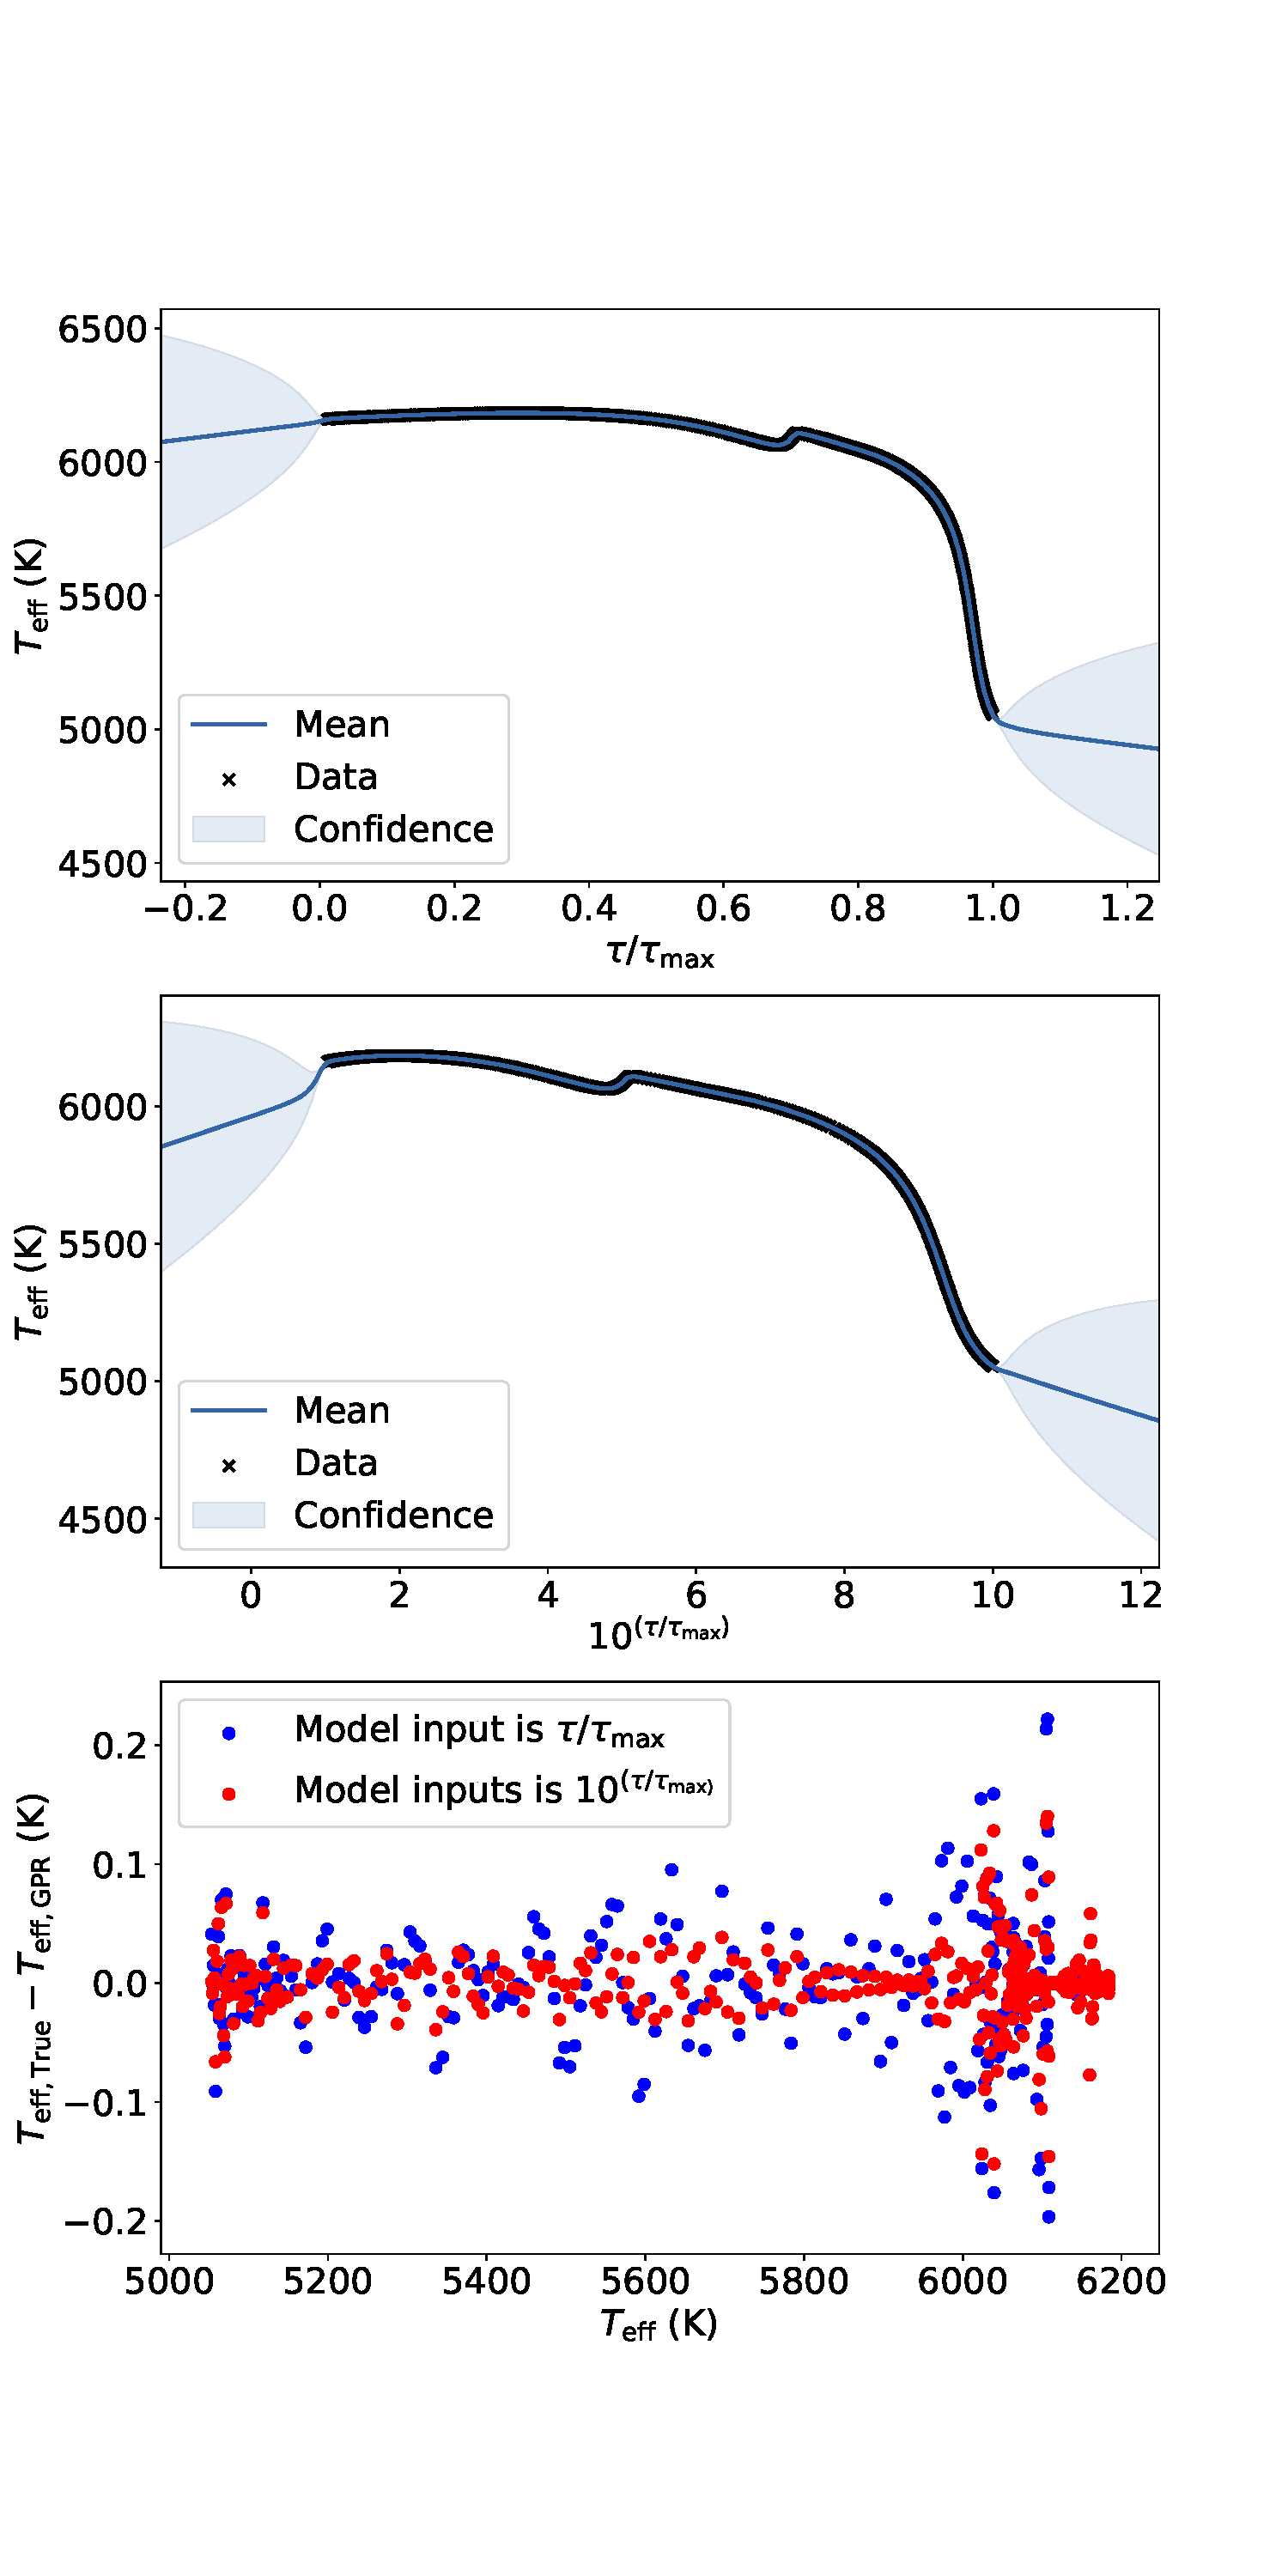
\includegraphics[width=1.0\columnwidth]{selection_of_t.pdf}
    \caption{The comparison between GPR model predictions with two different input age indices ($\tau/\tau_{\rm max}$ and $10^{(\tau/\tau_{\rm max})}$) for a 1.1$M_{\odot}$ track. Top: the GPR model of the effective temperature as a function of $\tau/\tau_{\rm max}$. The adopted kernel is MLP. Middle: same as the top, but the GPR model input is $10^{(\tau/\tau_{\rm max})}$). Bottom: residuals between true values and GPR model predictions. }
    \label{fig:selection_of_t}
\end{figure}
 

\subsection{Training Procdure}\label{workflow}
To demonstrate our work flow, we present our training process of a 2-demissions GPR model. The GPR model contents two inputs, namely, $M$ and $\tau'$,  and one output ($T_{\rm eff}$). We only adopted the stellar models with fixed [Fe/H]$_{\rm init}$ (0.0 dex), $Y_{\rm init}$ (0.28), and $\alpha_{\rm MLT}$ (2.1) from the primary grid. The total number of stellar models is 24,485. A validation data set was computed with the same model inputs but random masses. Our training procedure contents three major steps: data selection, model training, and model validation.      

\subsubsection{Step1: Data Selection}

As discussed in Section~\ref{grid}, we have three types of data for training, testing, and validating GPR models. The training data is apparently the model grid used to train GPR models.  The test dataset, which was also selected from the model grid but not used in any training processes. Test data are used to examine wether a GPR model gives proper description for the model grid. Once a GPR model provides good agreement with the testing data, the training succeeds. The last type is validation data, which are the off-grid models with random input parameters. Validation data are used to validate GPR models and also to estimate their systematical uncertainty. 

Because the computational and memory complexity exponentially increase with the number of data involved in the Gaussian Process. A practical limit of the training data is about 10,000. The testing and validation data could be massive but we set a limit of 50,000 for the efficiency.  This is to say, only a small subset of the model grid can be used. The sampling method is hence critical. The training data should uniformly cover the output ranges to avoid data gaps but also highly weight where quick changes occurs. %In our GPR model outputs, the five global parameters ($T_{\rm eff}$, $\log g$, $R$, $\delta \nu$, and $\nu_{\rm max}$) are tightly correlated during the evolution. They hence can be trained with the same data.
 Due to the \textsc{MESA} step-control strategy, stellar models are dense at the main-sequence and the red-giant phases but quite sparse on subgiant stage. Random sampling is hence not appropriate. We tested a few methods and found that using the displacement of each evolving step on the HR diagram as the weight gave the best sampling. The displacement is defined as $\delta d$ = $(\delta T_{\rm eff}^{2}$ + $\delta L^{2})^{1/2}$, where $\delta T_{\rm eff}$ and $\delta L^{2}$ are the differences between two consecutive models on the evolutionary track. We sampled on each evolutionary track separately and then combined the models as datasets. The sampling method gave a relatively uniform data distribution on the HR diagram and also highly weighted the regions around the hook and turn-off point.   
%
 %The data for the other two GPR outputs ($t$ and [Fe/H]$_{\rm surf}$) need to be separately sampled because of the evolutionary features.  
%
%The age mainly changes during main-sequence and slowly increases afterward. For this reason, we used the change of fractional age ($\delta t/t_{\rm max}$) at each step as the weight . The sampled data for training the age are hence much denser at the main-sequence than the evolved stages. 
% 
%The surface metallicity of an evolutionary track gradually reduces during main-sequence because of the element diffusion, however, rapidly increases at post main-sequence due to the quick expansion of the convective envelope. The training data ought to present evolving details at the giant phase and also properly cover that at the main-sequence. For this reason, we adopted the gradient of $(Z/X)_{\rm surf}$ as a function of the age index ($t'$) as the weight. We summarised the weight for a data point ($w_{i}$) on an evolutionary track as below:
%\begin{equation}\label{weights}
%w_{i} = \left\{\begin{matrix}
%\begin{aligned} 
 %& (\delta T_{\rm eff, i}^{2} + \delta L_{i}^{2})^{1/2} \; {\rm for}\;T_{\rm eff}, \log g, R, \delta \nu, {\rm and} \; \nu_{\rm max}, \\ 
%& \delta (Z/X)_{\rm surf, i}/\delta t' \;  {\rm for}\;(Z/X)_{\rm surf},\\ 
%& \delta \tau_{i}/\tau_{\rm max} \;  {\rm for}\;\tau.\\
%\end{aligned} 
%\end{matrix}\right.
%\end{equation}
%
%The test and validation data should uniformly cover the HR diagram for sensible statistical results. We hence used the sampling method for the five global parameters in Equation~\ref{weights} for these two types of data. 
%
We demonstrated our selection for data to train the 2-demission GPR model ($T_{\rm eff}$ = $f(M, t')$) in Figure~\ref{fig:data_on_hrd}.  Here we sampled 3,000 and 5,000 on-grid models as the training and test data, and 5,000 off-grid models as validation data.  

\begin{figure}
	\includegraphics[width=1.0\columnwidth]{2D_data_on_HR.pdf}
    \caption{Selected training and testing data for the GPR model with 2-demission inputs on the $T_{\rm eff}$ - $\log g$. Black, blue, and red dots represent training, test, and validation data. }
    \label{fig:data_on_hrd}
\end{figure}

\subsubsection{Step 2:  Model Training}

In the model training step, we applied a data-residual process, which is described as follow. 
A GPR model (M0 here after) is primarily trained with the training data and tested with the test data. If residuals of test data are significant large or present any local structures, an extra GPR model (M1 hereafter) will be trained to describe the first-order residuals. With M0 + M1, the second-order residual could be calculated and used to train another extra GPR model (M2 hereafter). The training process goes to $n$-order residuals (M$n$) until GPR predictions do not significantly improve. Thus, the process provides a series of GPR models as a combination to describe stellar evolutions. Here we illustrated the details the process by training the 2-demission GPR model ($T_{\rm eff}$ = $f(M, t')$). 

We firstly train the primary GPR model (M0) with the training dataset shown in Figure~\ref{fig:data_on_hrd}. We used the MLP kernel and optimise M0 with random initial hyperparameters. The result of M0 is demonstrated in Figure~\ref{fig:gpmodel}. It can be seen that the GPR model has transferred the model grid into a continued function (indicated by contour lines). For models below $\sim$1.05$M_{\odot}$, the $T_{\rm eff}$ contour lines are smooth and the GPR model give good description for the data. However, the structure becomes complex at $t'\sim5$ when $M$ is larger than 1.05 because of the appearance of the 'hook' in stellar evolution. And the GPR model predictions does not very convinced in this area. This can be seen in the left bottom panel in Figure~\ref{fig:drprocess}, which shows the offsets between M0 predictions and the test data (testing errors hereafter). The large offset in the local area indicate M0 does not well describe the whole grid. This is because we only used a small subset for training and did not pass enough details for the GPR model to learn. It is a common issue with the Gaussian process when training big data set because of the limitation of the size of training data. To mange this issue, we developed the data-residual process aiming to use multiple GPR models to describe the grid. This process is illustrated in Figure ~\ref{fig:drprocess}. After training and testing M0, we trained an extra GPR model (M1) to describe the 1st-order residuals. We randomly selected 20,000 on-grid models, used M0 to predict their effective temperature, and calculated 1st-order residuals. We then sampled 3,000 training data from these 20,000 models weighting by their absolute residual values, saying that models with large offsets were highly-weighted. The selected training data for M1 is presented in the top middle graph. As it can be seen that the area where M0 does not well describe are highlighted with more dense data points than other regions. The training of residuals are operated with a kernel competition because we can predict which kernel would work. We trained 5 GPR models with MLP, RBF, RQ, EXP, and Mat32 kernels, combined each of them with M0, and computed testing errors. Because M1 mainly focuses on improving the poor prediction in small regions (a few percent of the dataset). We quantified absolute testing errors with two cumulative values at 95\%, and 99.8\%.  The 99.8\% cumulative value was firstly compared to decide the best kernel. If there was no obvious differences (< 5\%),  the 95\% value would be used. In the presented example, the MLP kernel won and the corresponding model was selected as M1. We presented the testing errors for M0+M1 in the bottom middle panel. Those large offsets significantly reduce and the error distribution turns to be random. With the same approach for M1, we trained M2 for the 2nd-order residuals and tested the model combination of M0+M1+M2. However, the improvement of testing errors (bottom right) was very small (<5\% for both 95\% and 99.8\% cumulative values), and we hence terminated our training process. Here we obtained a GPR model combination to describe $T_{\rm eff}$ as a function of $M$ and $\tau;$. 
%

As demonstrated above, the data-residual process is able to break through the limitation of training data by separating data features into the general and the local levels. In this example, although we set up a limitation of 3,000, the actual data points involved in the training process was around 7,000 (considering the overlapping of three GPR models). The other advantage of this process is offering flexibilities to manage different evolving features of outputs. For instance, quickly changes appear around the hook for the effective temperature but at the subgiant phase for the surface metallicity. The data-residual process allows the training to focus on different local areas in the parameter space for different outputs when dealing with residuals.   

\begin{figure}
	% To include a figure from a file named example.*
	% Allowable file formats are eps or ps if compiling using latex
	% or pdf, png, jpg if compiling using pdflatex
	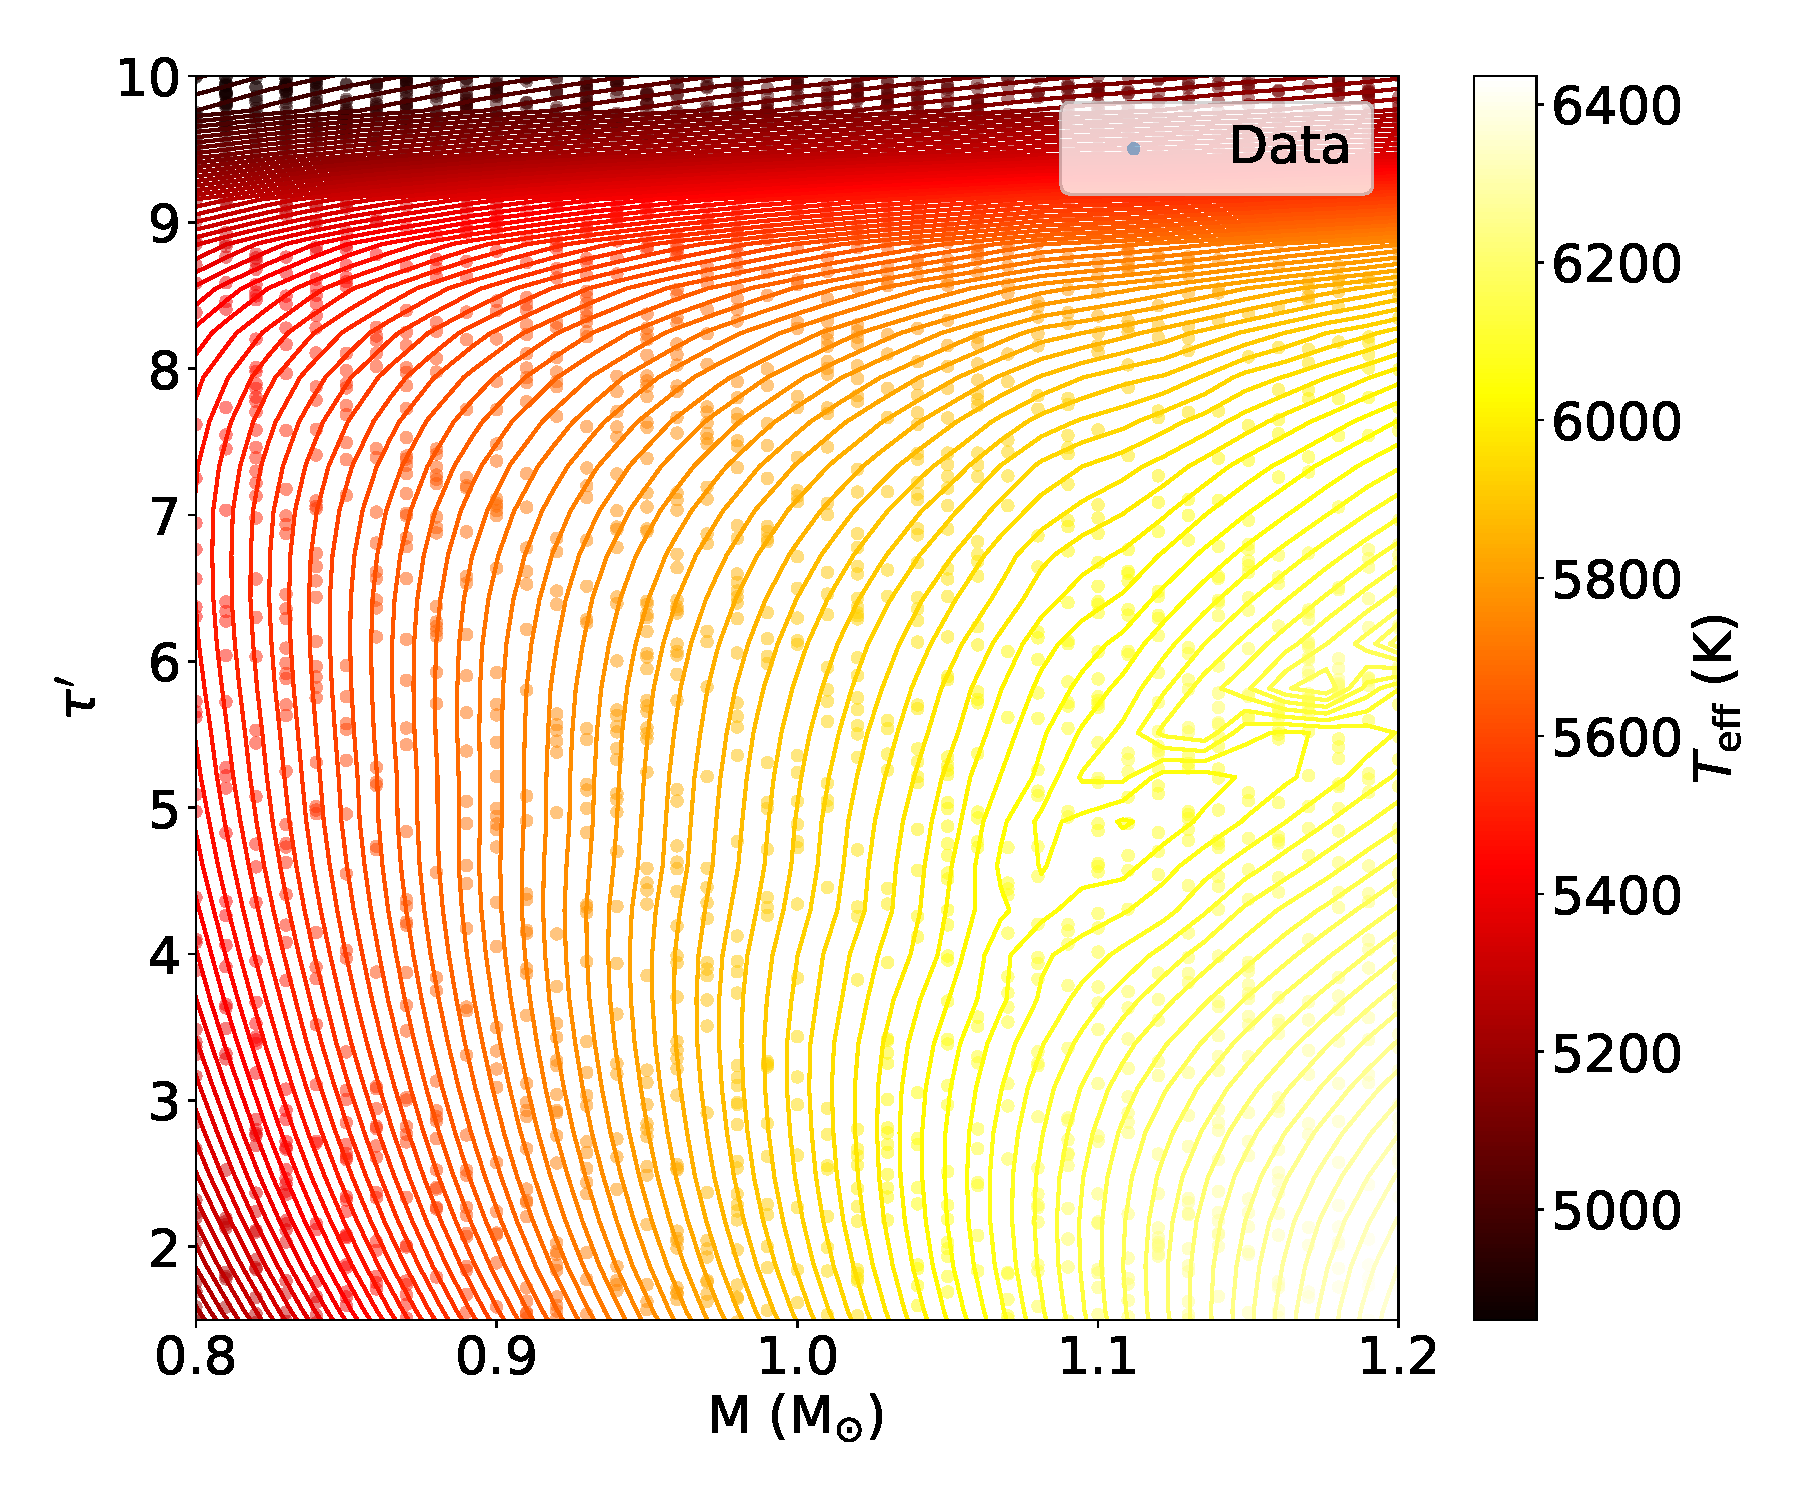
\includegraphics[width=1.0\columnwidth]{2d_gpmodel_MLP.pdf}
    \caption{Top: The GPR model (using the MLP kernel) for the effective temperature ($T_{\rm eff}$) as a function of mass ($M$) and age index ($t'$). Dots represent the training data and counters indicate the GPR predictions. }  
    \label{fig:gpmodel}
\end{figure}


\begin{figure*}
	% To include a figure from a file named example.*
	% Allowable file formats are eps or ps if compiling using latex
	% or pdf, png, jpg if compiling using pdflatex
	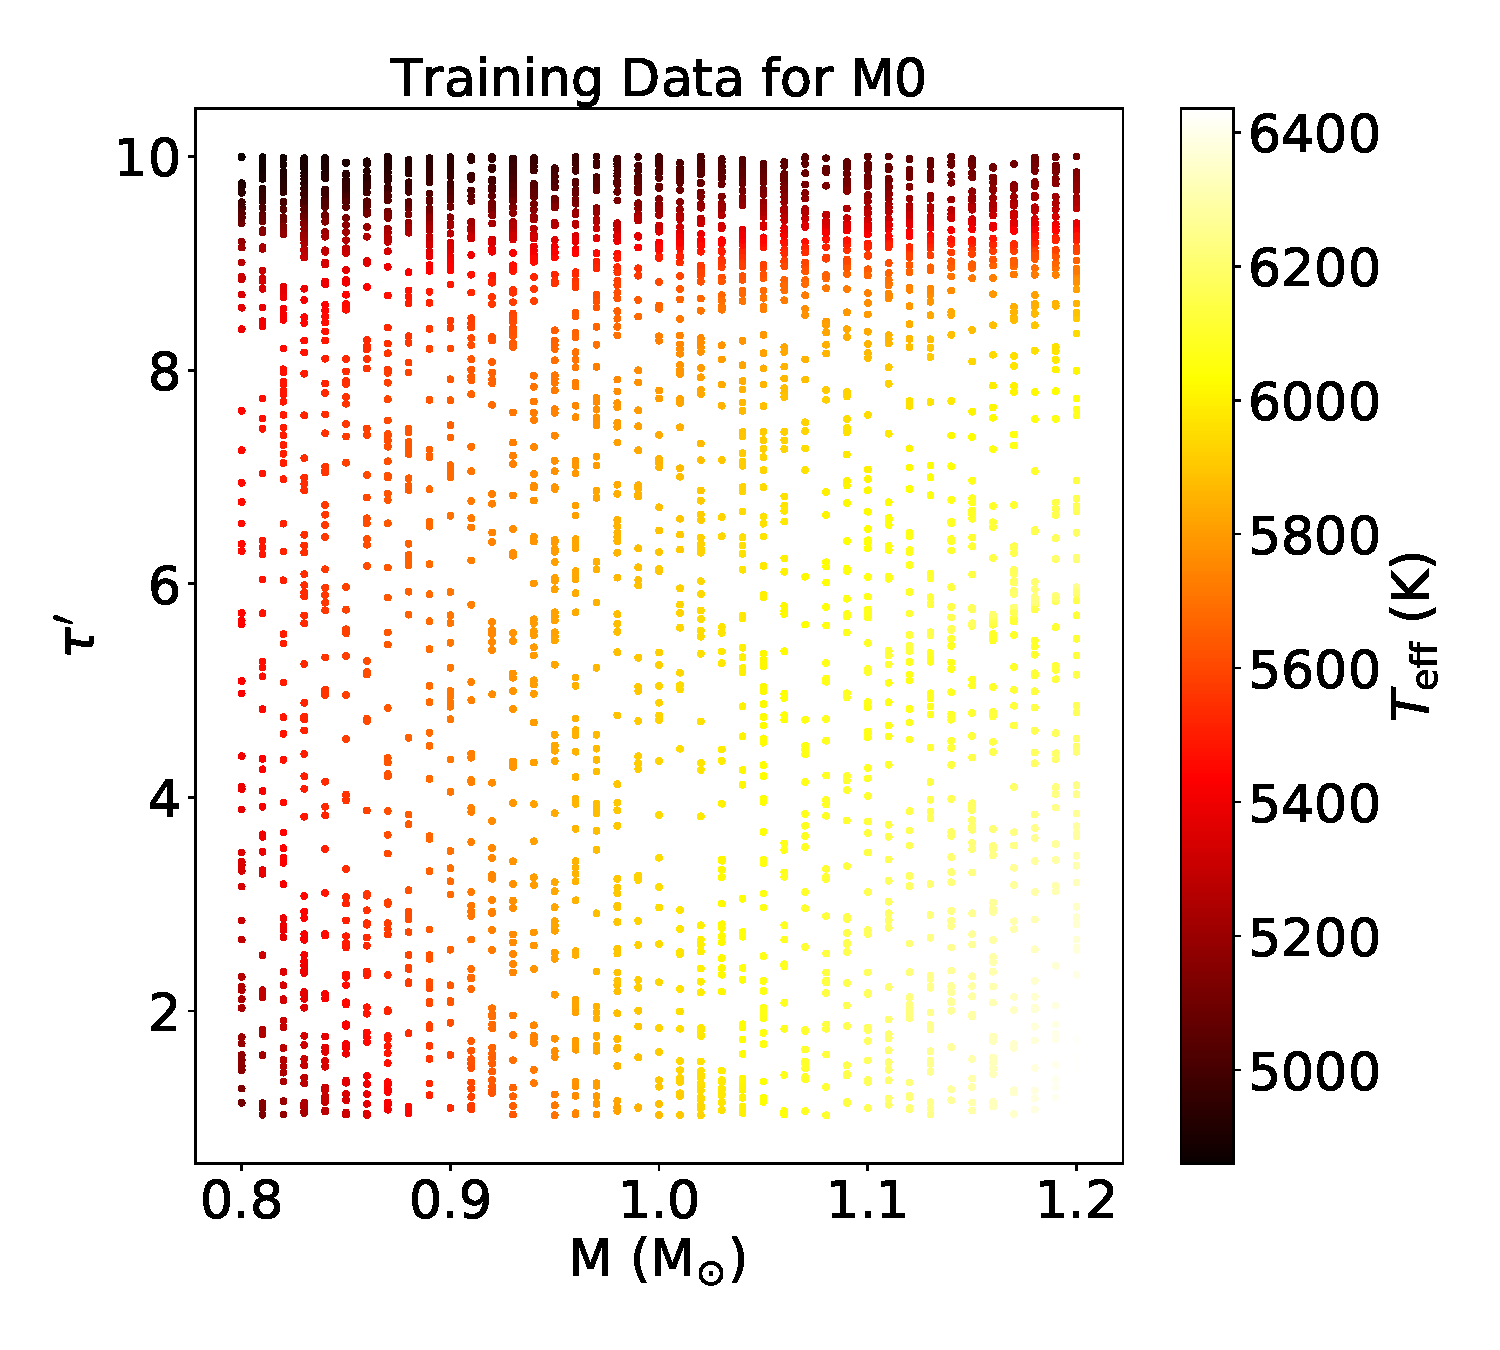
\includegraphics[width=0.33\textwidth]{M0_data.pdf}	
	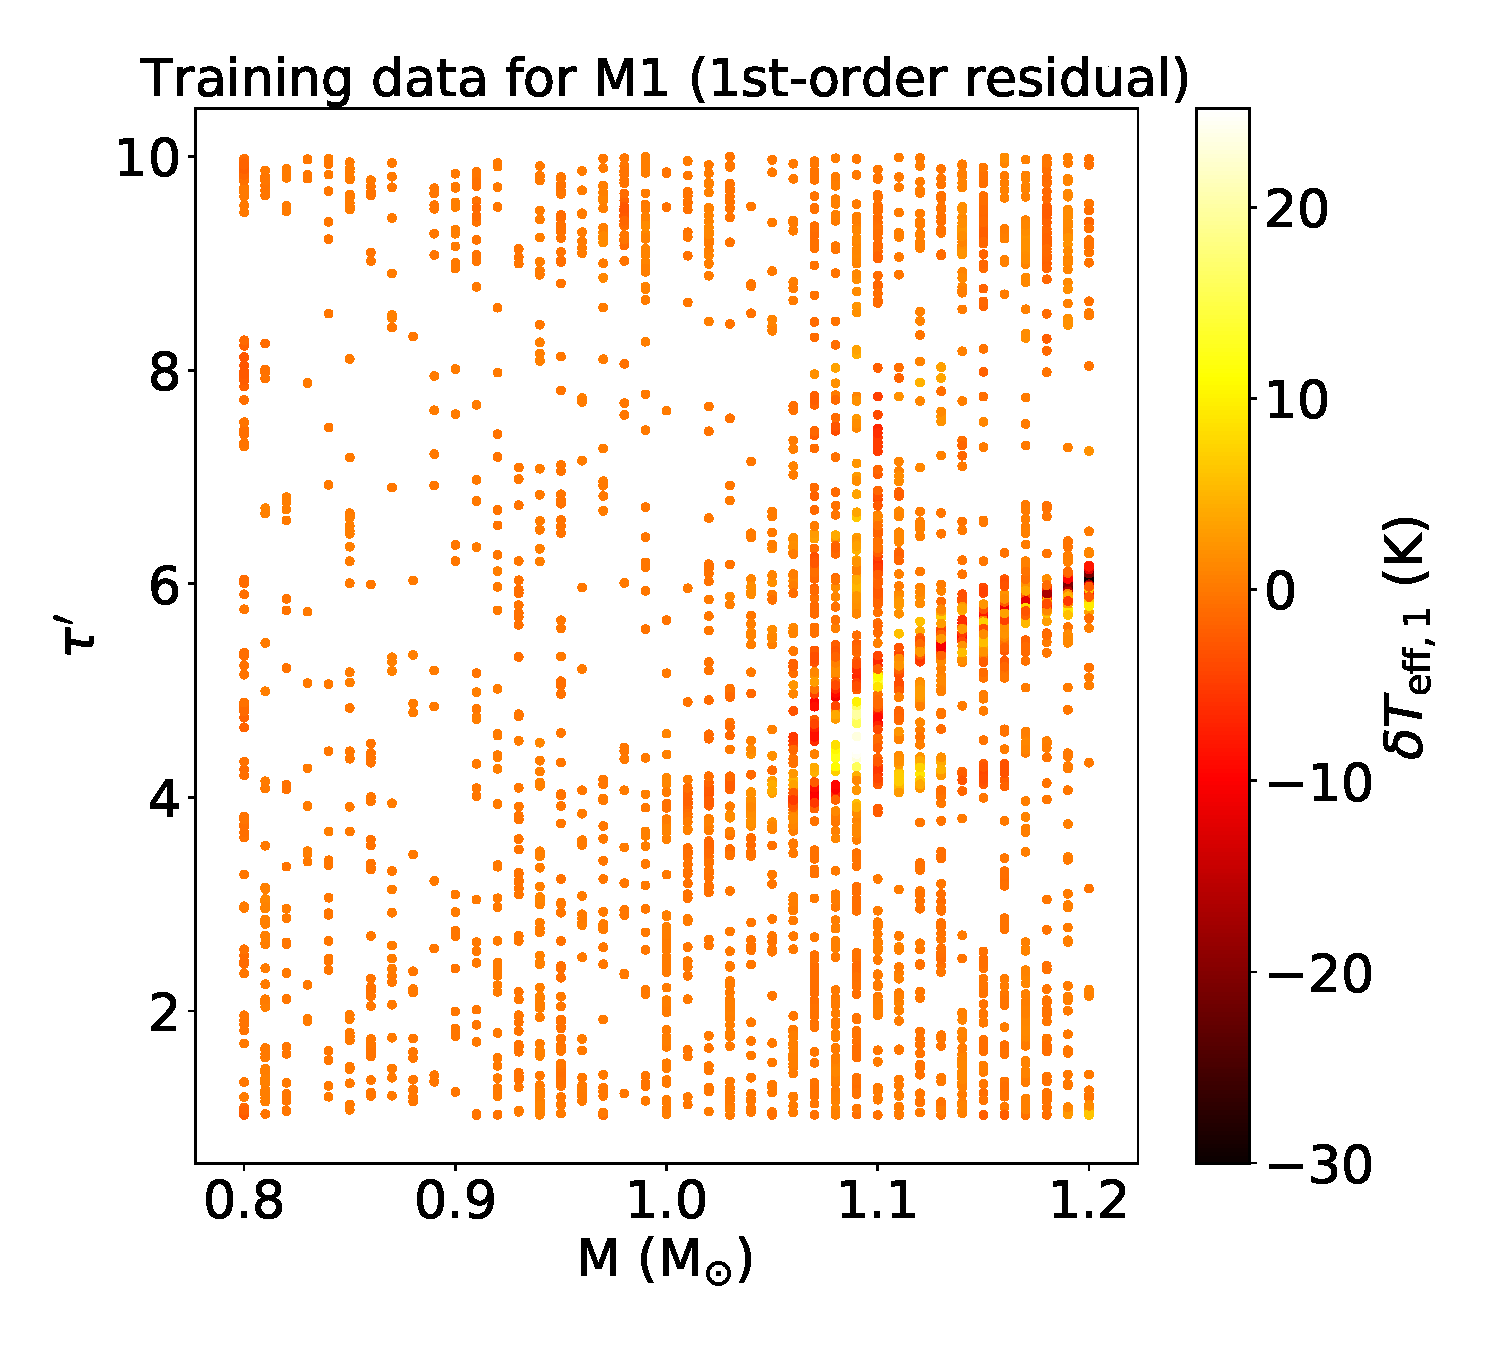
\includegraphics[width=0.33\textwidth]{M1_data.pdf}
	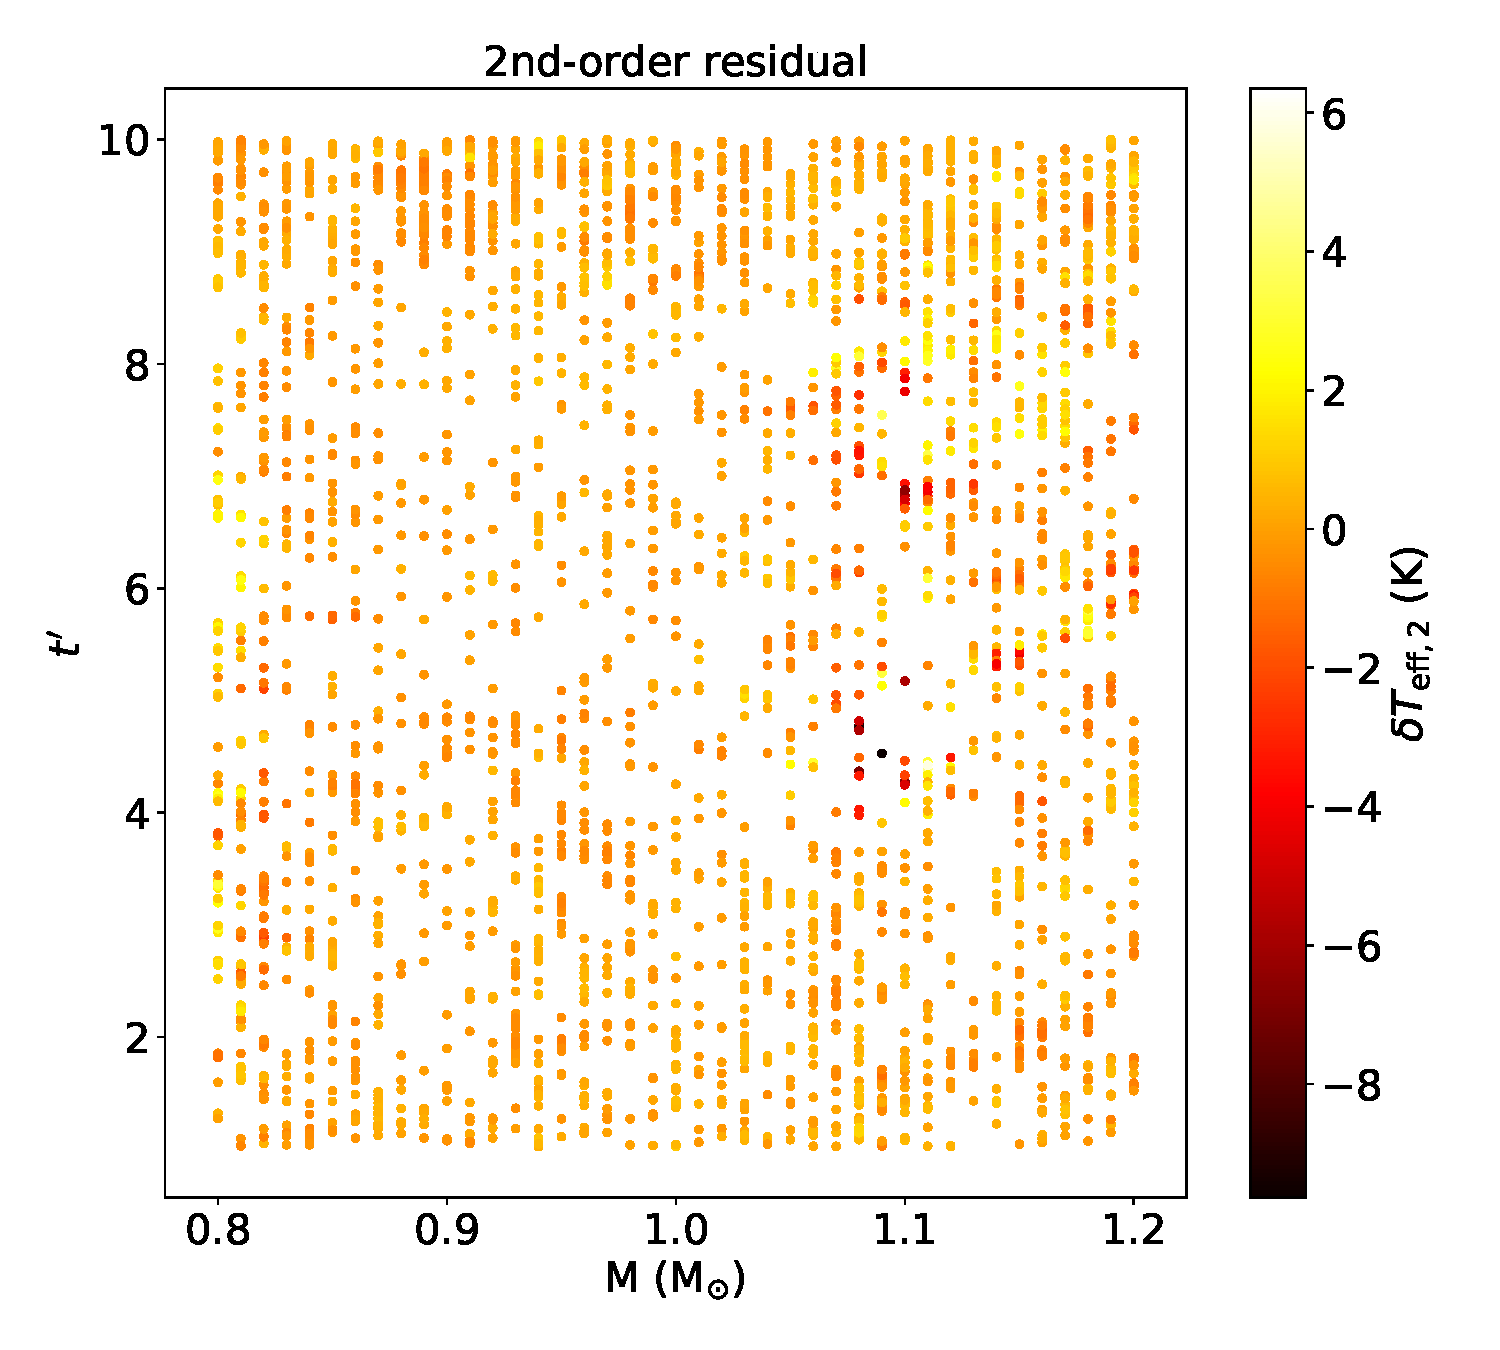
\includegraphics[width=0.33\textwidth]{M2_data.pdf}
		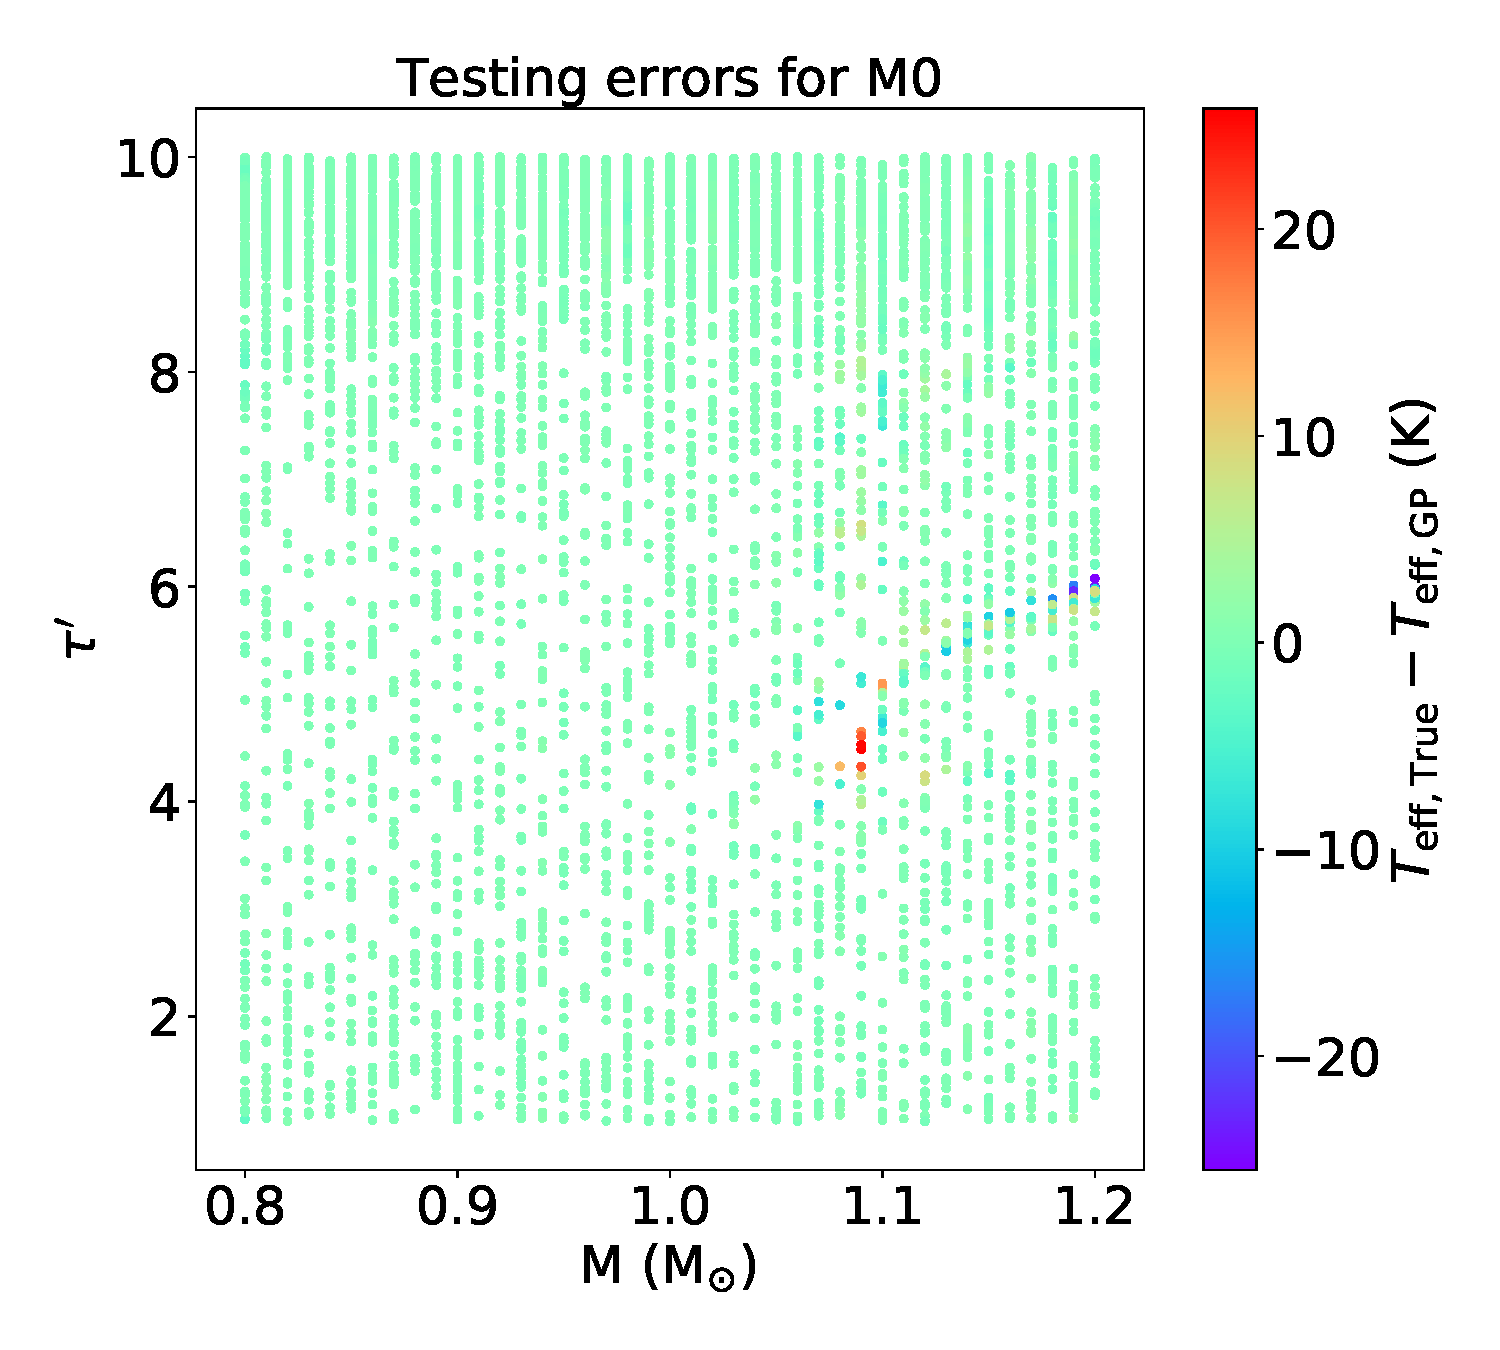
\includegraphics[width=0.33\textwidth]{M0_test.pdf}	
	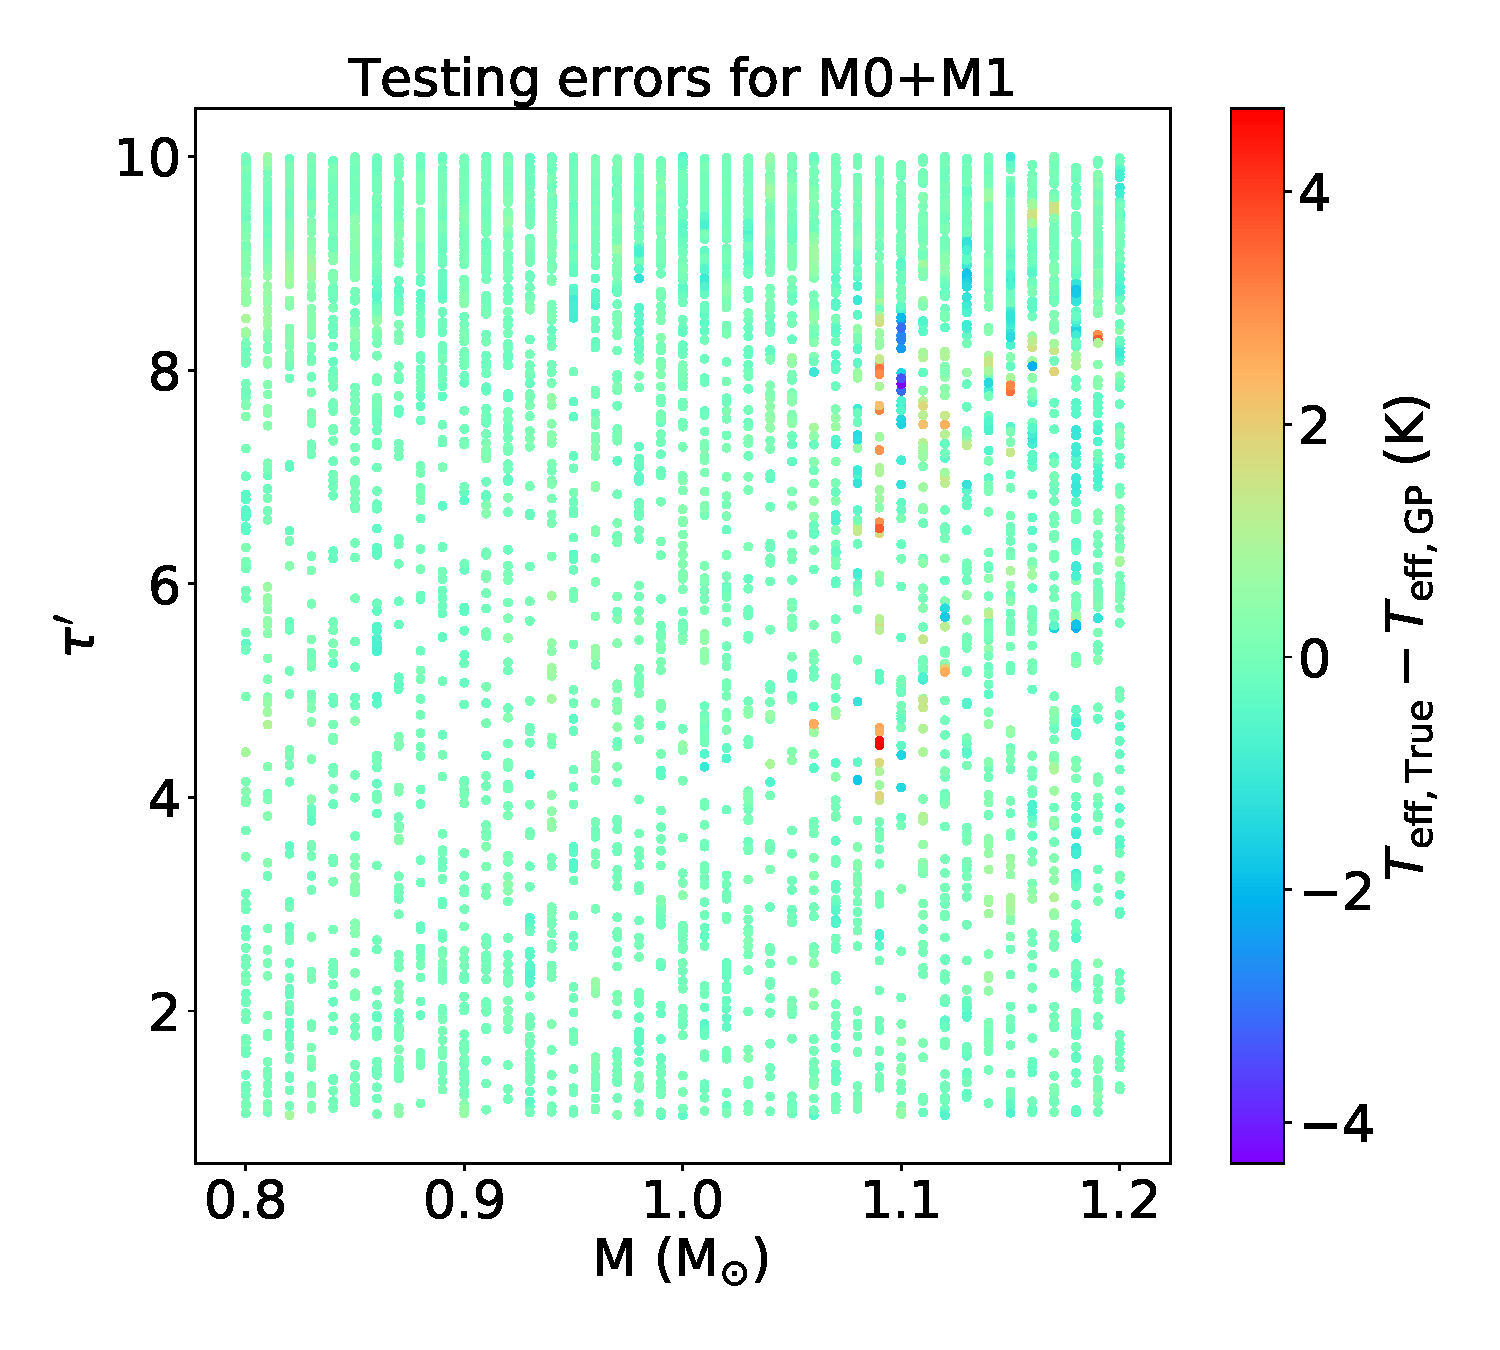
\includegraphics[width=0.33\textwidth]{M1_test.pdf}
	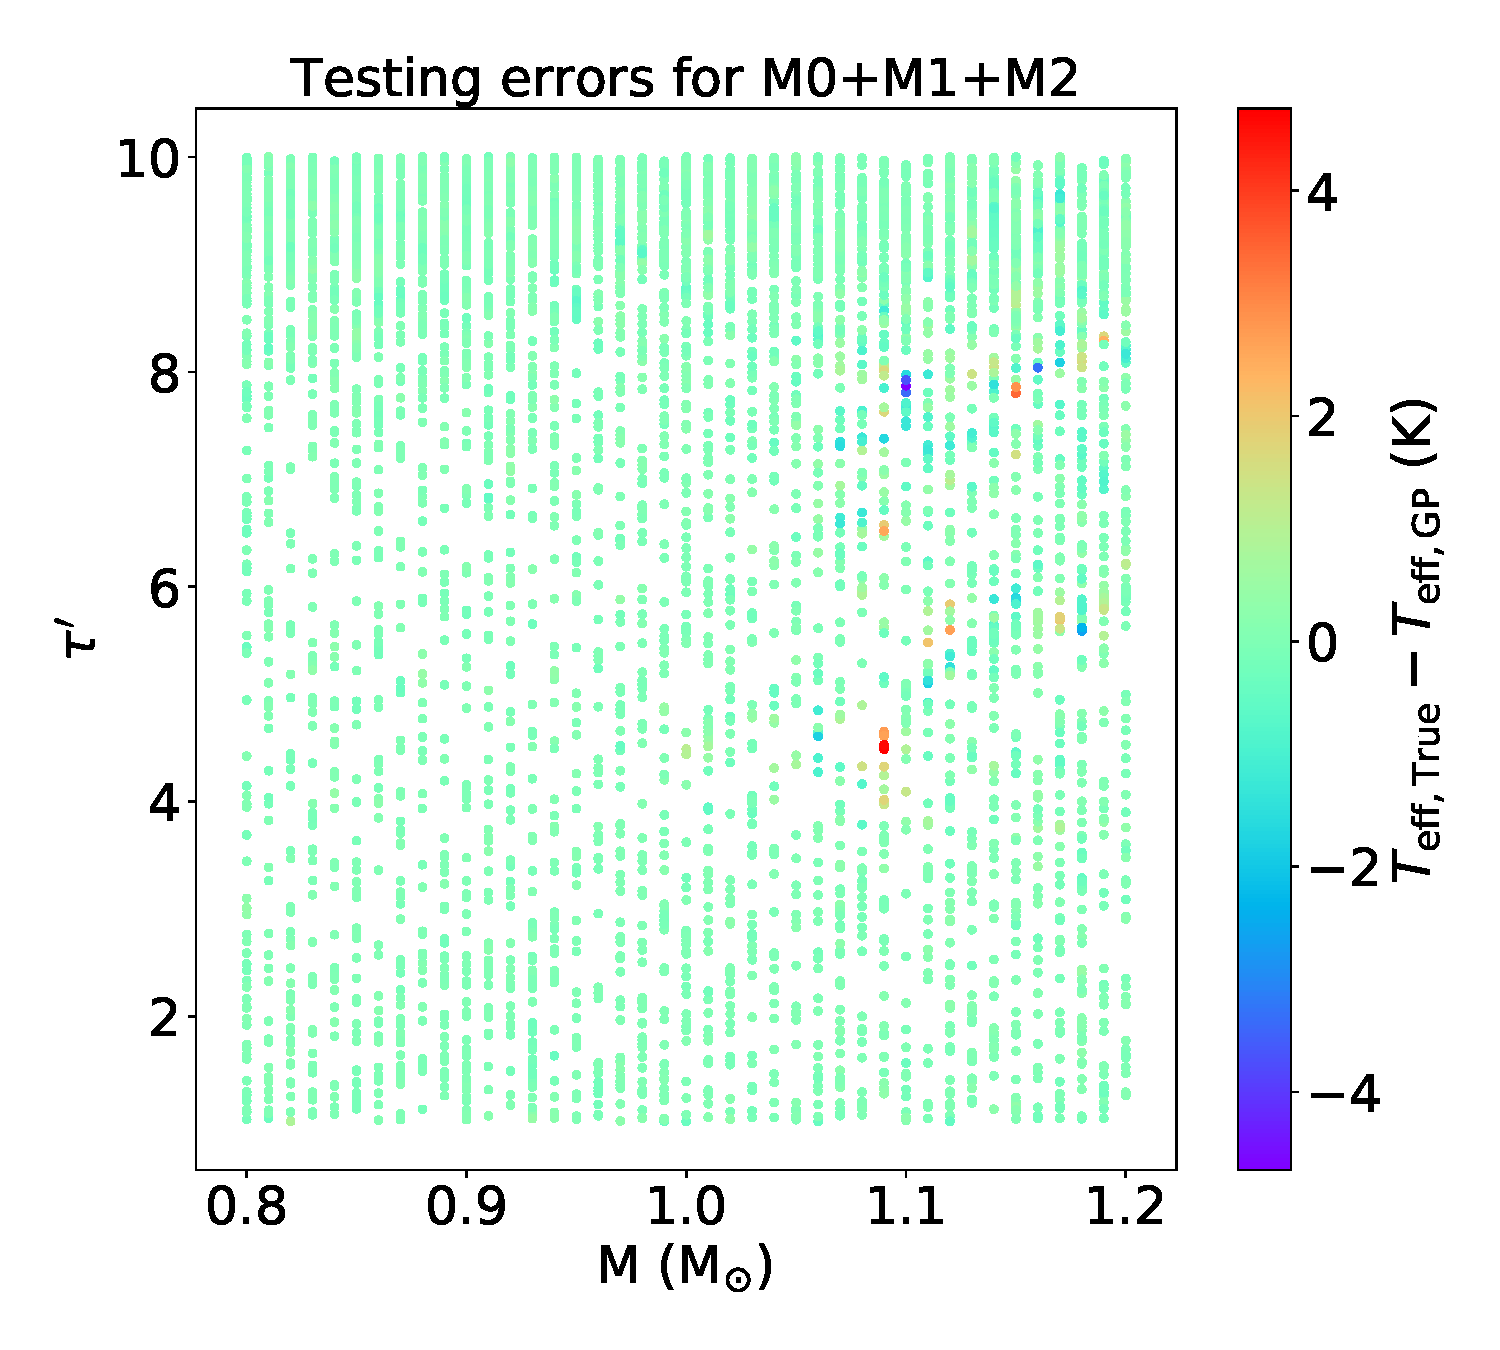
\includegraphics[width=0.33\textwidth]{M2_test.pdf}
    \caption{The data-residual process for training the 2-demission GPR models for the effective temperature. The top row (from left to right) shows the training data used to train the data (M0), the first-order residuals(M1), and the second-order residuals(M2). The bottom row (from left to right) demonstrates the reduction of testing errors along the training process.}  
    \label{fig:drprocess}
\end{figure*}

% \begin{figure}
	% To include a figure from a file named example.*
	% Allowable file formats are eps or ps if compiling using latex
	% or pdf, png, jpg if compiling using pdflatex
%	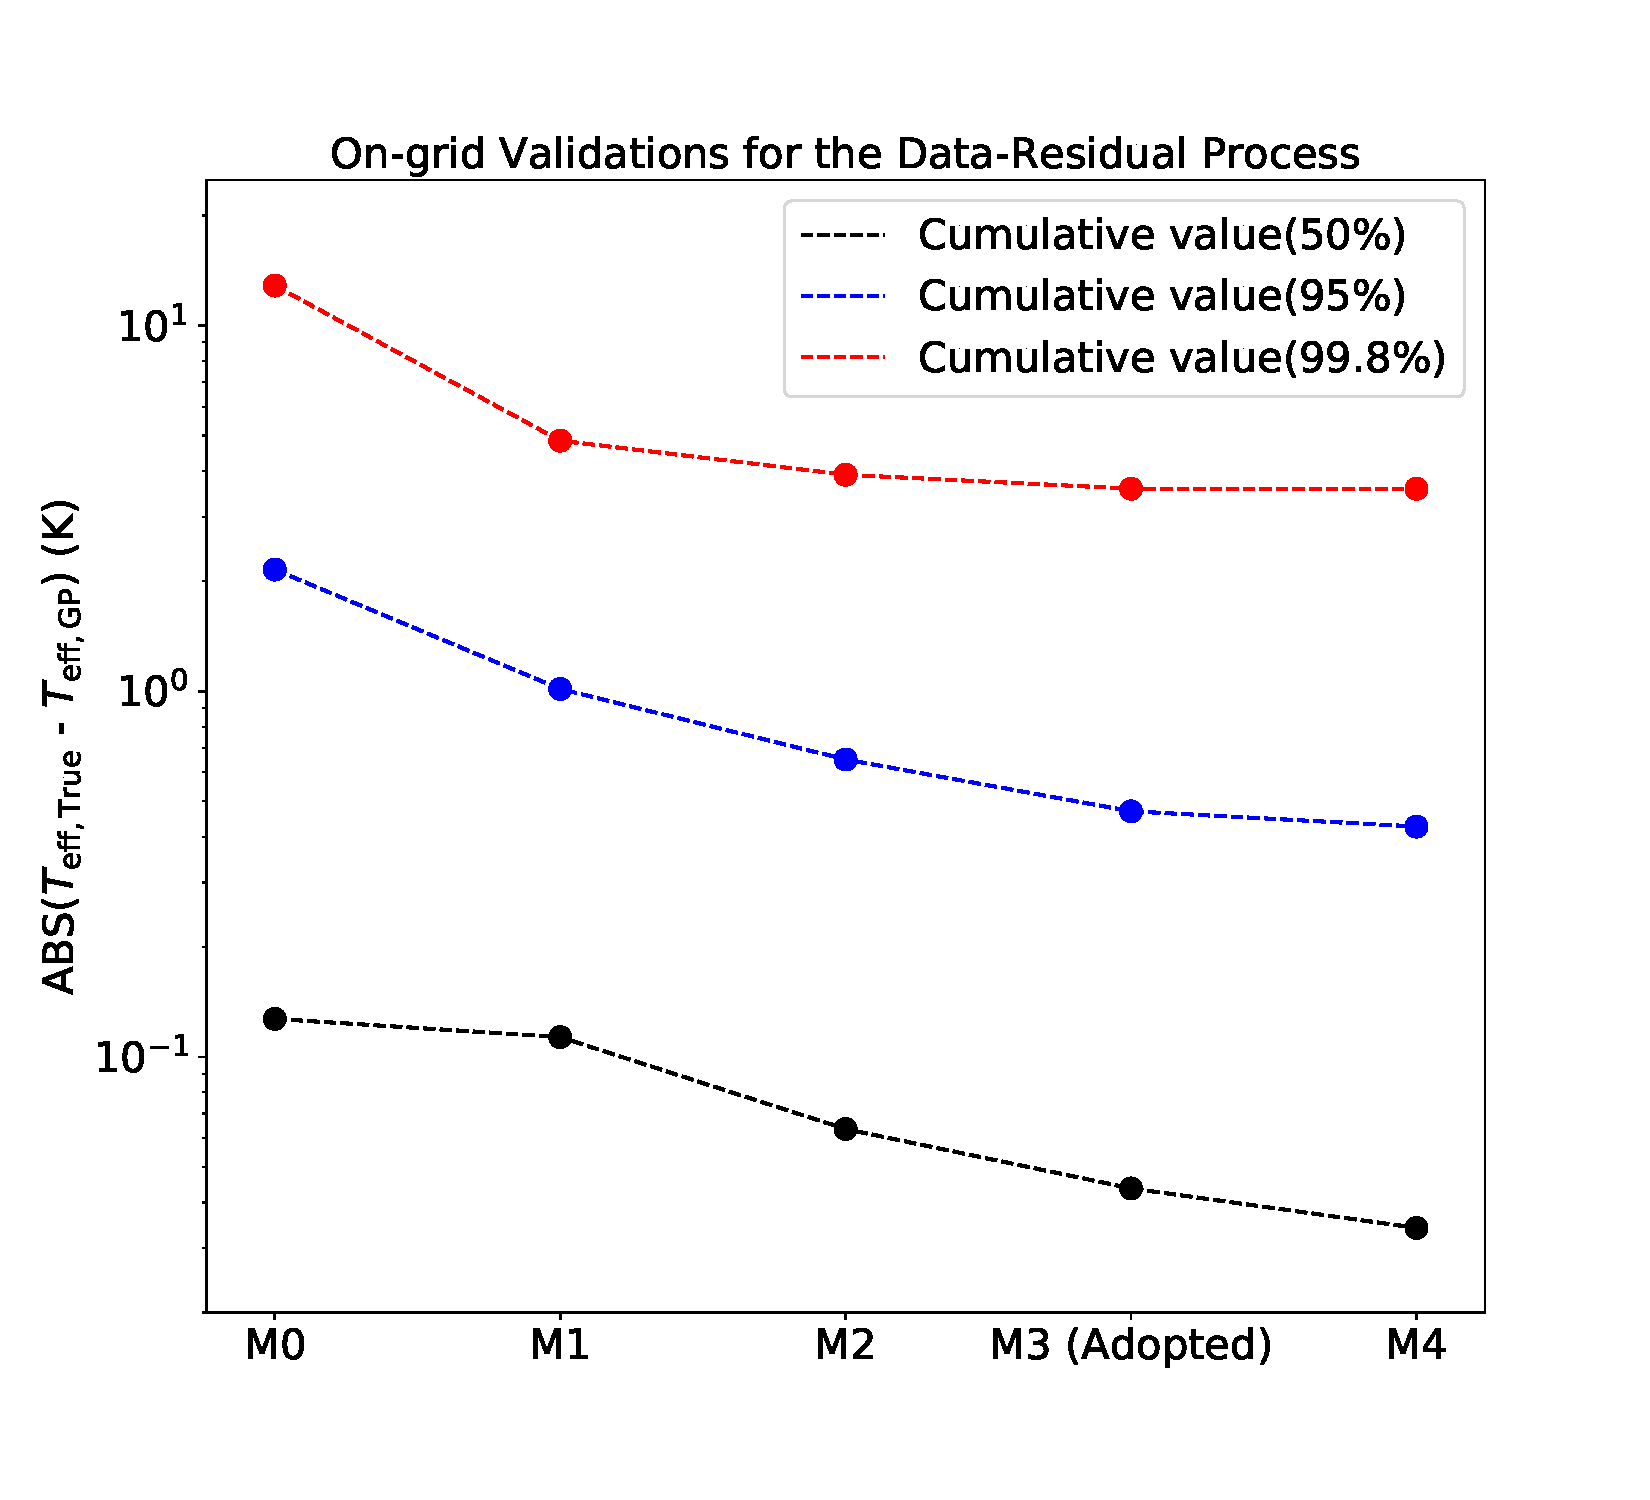
\includegraphics[width=1.0\columnwidth]{all_validations.pdf}
%    \caption{On-grid validations.}  
%    \label{fig:on-grid_validation}
%\end{figure}

\subsubsection{Step 3: Model Validation}

We lastly validated the GPR models by using the offsets between GPR predictions and the validation data (validation errors here after).  We quantified absolute validation errors with three cumulative values at 50\%, 95\%, and 99.8\%. The first two are used to validate GPR models in general level. The last value is used to validate those evolutionary phases where GPR models do not work well. Because a large deviation between the 95\% and 99.8\% cumulative values often means a long tail of probability distribution, which indicates that GPR models poorly describe some local areas. In Figure~\ref{fig:off-grid_validation}, we demonstrated the validation errors for the model combination obtained above. As It can be seen that, the GPR models well predict $T_{\rm eff}$ in most area, however, not very well match those around M$\sim1.1M_{\odot}$ and $\tau'\sim5$ (the main-sequence the hook). Comparing with the testing errors in Figure \ref{fig:drprocess}, the validation errors indicate that although the GPR models were well trained to describe the model grid in this area, they still do not learn the feature between the grid. The reason is that $\sim1.1M_{\odot}$ the boundary between tracks with and without the 'hook'. The local structure is hence more complex than any other areas (as it can be seen in Figure \ref{fig:gpmodel}) and it leads to relatively poor predictions. Because the distribution of validation errors in the input space is not flat, it is difficult to measure a global systematical uncertainty. We will discuss how we applied systematical uncertainty when fitting stars in Section \ref{sec:augmentation}. 
 
 
 \begin{figure}
	% To include a figure from a file named example.*
	% Allowable file formats are eps or ps if compiling using latex
	% or pdf, png, jpg if compiling using pdflatex
	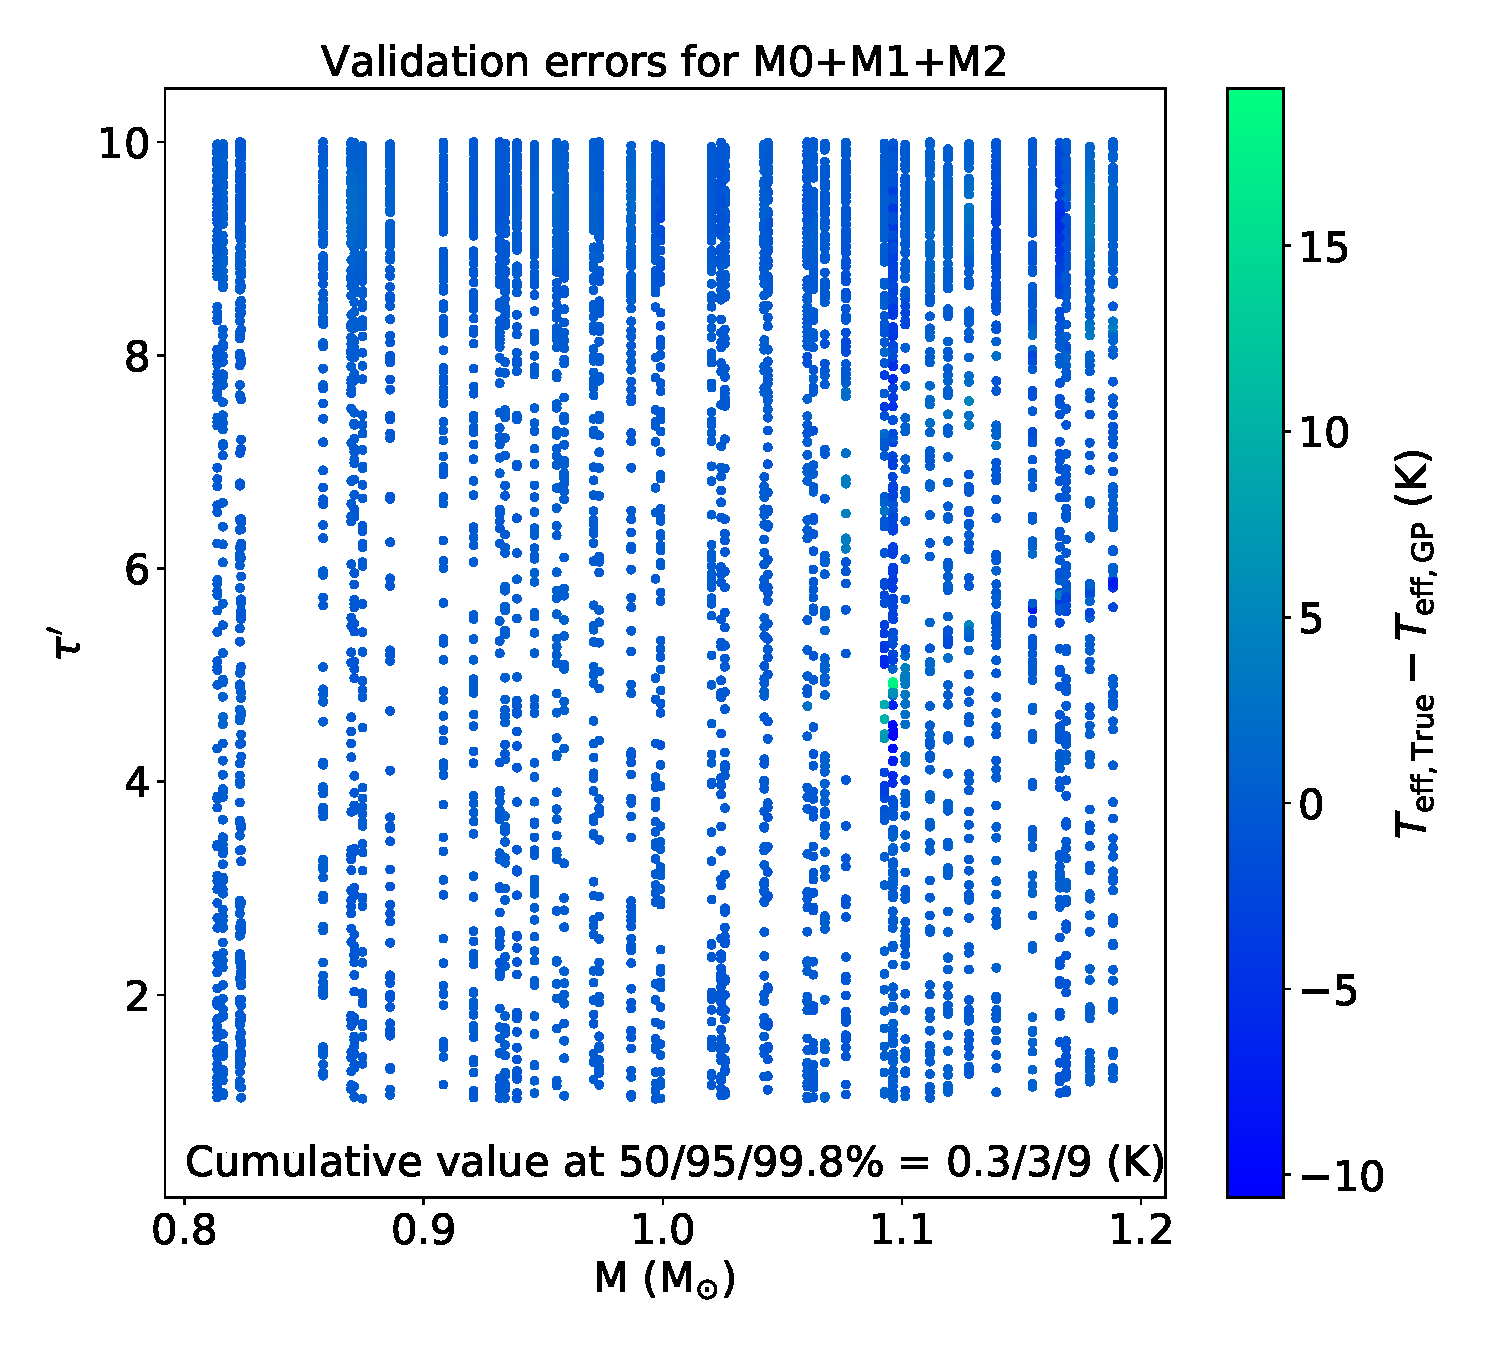
\includegraphics[width=1.0\columnwidth]{off_validation.pdf}
    \caption{Validation errors of $T_{\rm eff}$ on the $M-\tau'$ diagram for the 2-demission GPR models ($T_{\rm eff} = f(M, \tau')$).}  
    \label{fig:off-grid_validation}
\end{figure}

\subsubsection{Summary of the Training Procedure}
Here we summarised our training procedure. We firstly selected three types of data for training, testing, and validating GPR models. The sampling method of training data are different for the outputs depending on their evolving features. The test and validation data were sampled uniformly on the HR diagram to equally cover all evolutionary stages. We then trained GPR models with given inputs and outputs following a data-residual process. A primary model is trained to describe the general feature of the grid, and some extra models are then trained to reveal local structures. A combination of these GPR models is used to describe the \textsc{MESA} grid. Model validation is lastly carried out to validate GPR models and also to estimate systematical uncertainties. With the training process, we trained 2-demission GPR models for $T_{\rm eff}$ and $\log g$, and used them to make a non-sparse $T_{\rm eff}$ - $\log g $ diagram as shown in Figure \ref{fig:gphrdl}. 
 
\begin{figure}
	% To include a figure from a file named example.*
	% Allowable file formats are eps or ps if compiling using latex
	% or pdf, png, jpg if compiling using pdflatex
	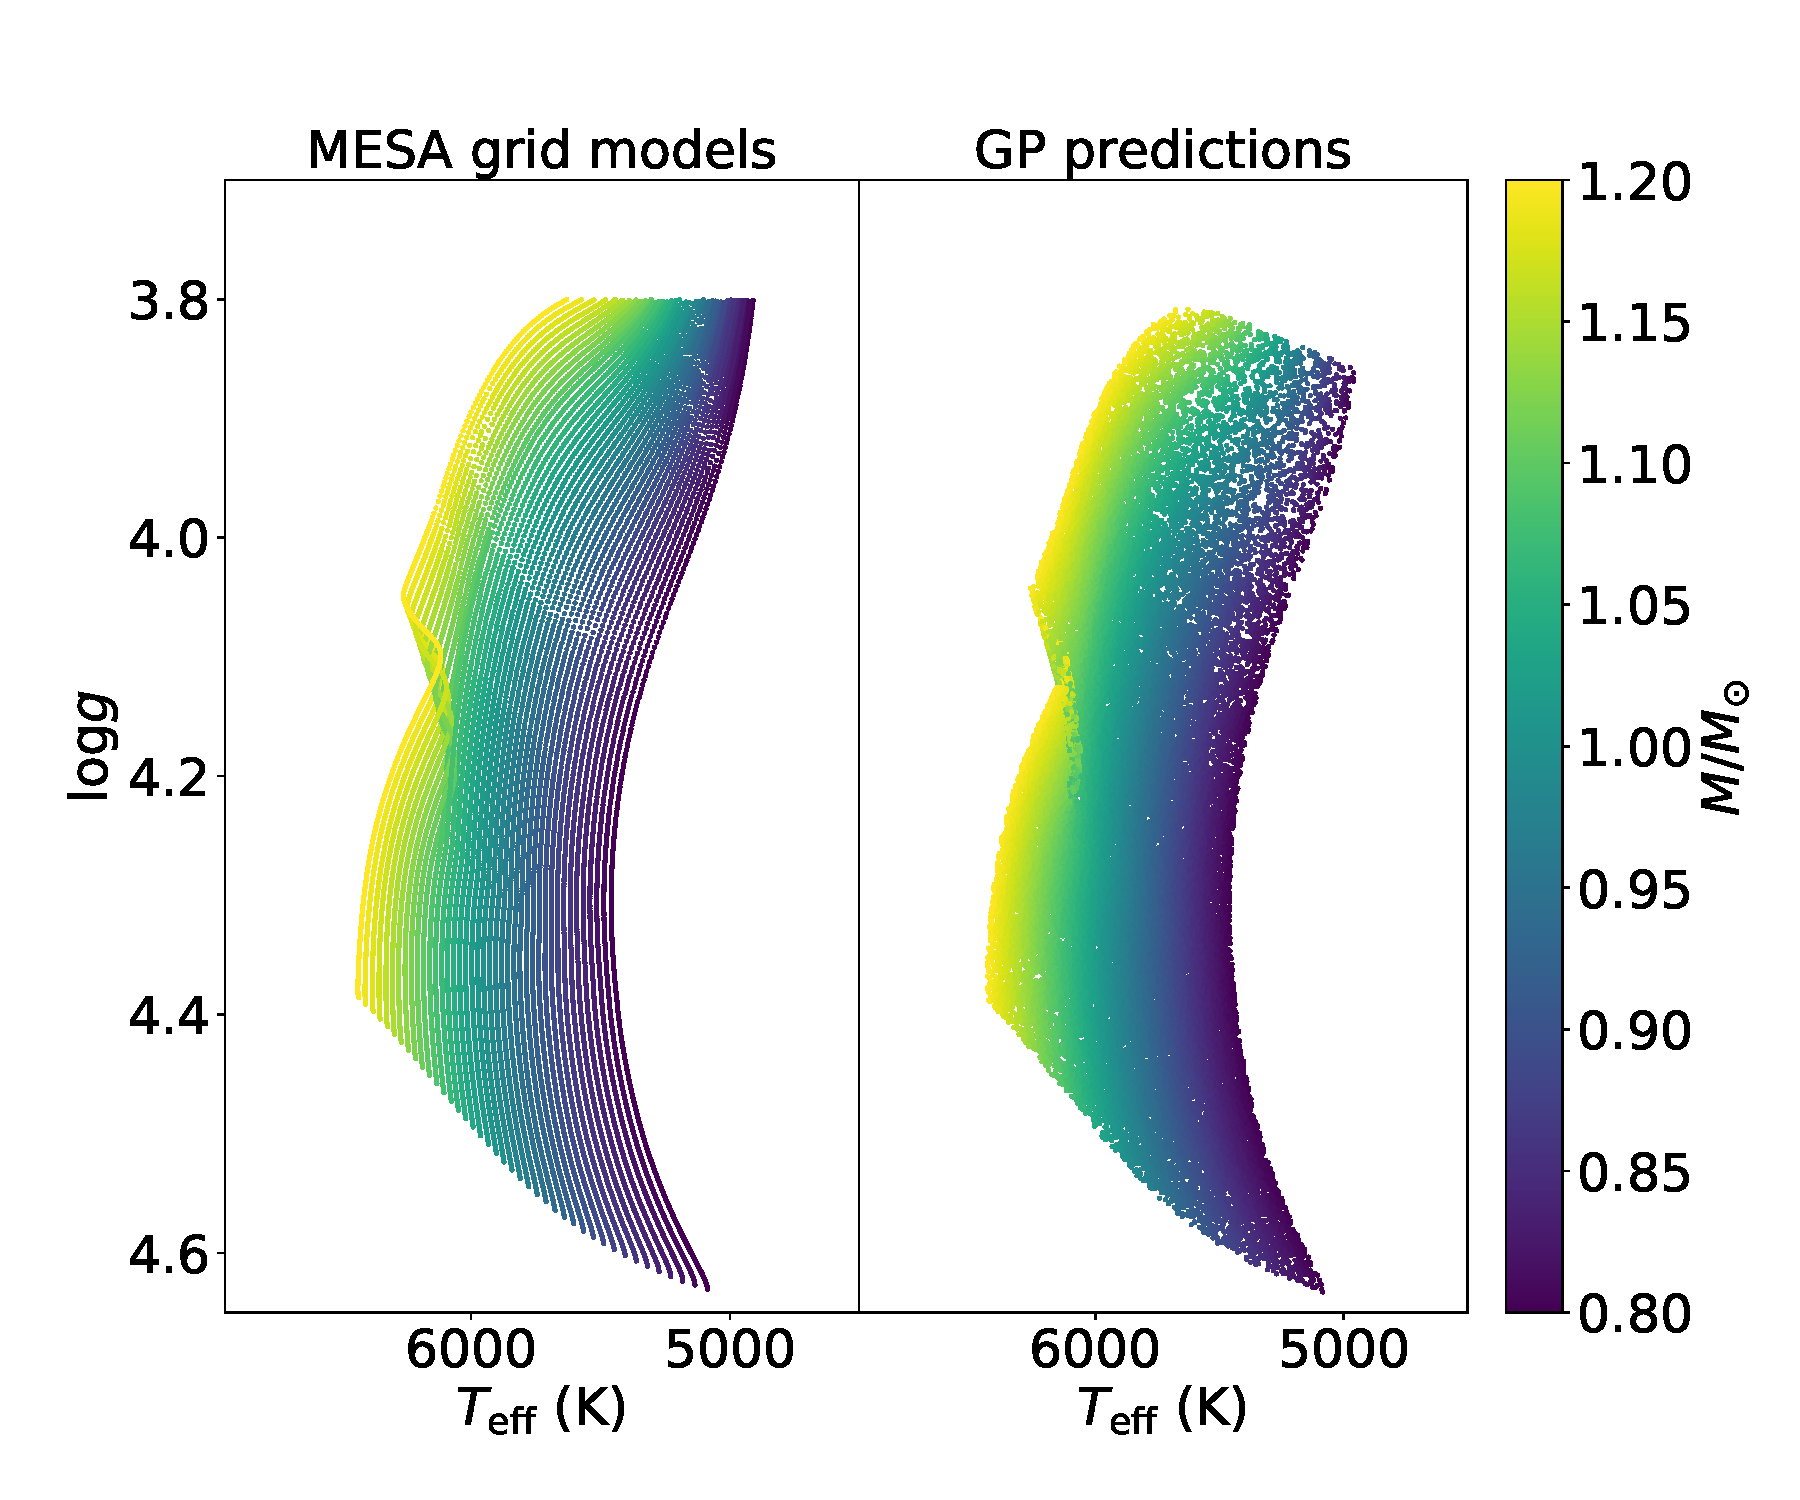
\includegraphics[width=1.0\columnwidth]{2d_hrd_compare.pdf}
    \caption{MESA grid models (sparse) and GP predictions (non-sparse) on the $T_{\rm eff}$ - $\log g$ diagram. Note that we only predict models with $\log$ >= 3.8 to avoid the edge effect. }
    \label{fig:gphrdl}
\end{figure}




\section{Augmenting the MESA Grid}\label{sec:augmentation}

With the GP model described in Section \ref{GPR},  we train GP models for the MESA grid. The training data includes the primary and the additional girds as mentioned in Table~\ref{tab:grid}. The role of the additional grid is increasing the grid resolution for the high-mass models with hooks. As discussed in the previous section, the kernel function in the 'hook' area are much more complex than other regions , and hence a GP model requires more information to map the feature in this region. The total training data includes $\sim$ 15,000 evolutionary tracks and $\sim$ 10,000,000 data points. For validating and testing the data, we computed another 4880 tracks with random model inputs within the grid ranges. These tracks are split 50-to-50 for validating (in the training progress) and testing (after the training progress) GP models. We used the same sampling method of training, validating, and testing data. For each EEP section, we use 20,000 training data points and 20,000 validating data in the training progress.The testing data are selected in the whole EEP range and we use 50,000 (out of $\sim$1,000,000) data points. Note that we do not use models with $\tau \geq$ 20.0 Gyr, [Fe/H]$_{\rm surf} \leq$ -0.6 dex, or $T_{\rm eff} \geq$ 7000$K$ as testing data.    

\subsection{Overall Results}

We firstly train an Exact GP model for the whole grid with 20,000 model, corresponding to a sampling rate of $\sim$0.2\%. The testing indexes of outputs remarkably increase compared to those of 3D GP models. We listed the testing errors of this 5D GP model in Table~\ref{tab:results}. Results of 2D and 3D GP models are also given for comparisons. It shows clear decline in GP model accuracy with increasing input demission. 
%
We then train GP models with the section scenario. We gradually increase the number of sections and track changes in testing errors. We found that improvements in testing errors becomes not significantly when the section number goes above 10. As it shown in Table~\ref{tab:results}, the 68th and 95th testing errors are at same accuracy levels for sections more than 10. Although the 99.7th errors seem to be better with more sections, this is more like a random error given the change is a small fraction. 
%
It turns out that the most efficient sampling rate is around 1\% (10 sections). Above this rate, GP models learn no additional information about the grid. (references about this point?) 
%
Because less sections means less time and memory consumed for predicting. When take the 10-sections GP model as the final solution. Following analysis are all done with this model.   


\begin{table*}
	\centering
	\caption{Training and validating errors for GPR Models}
	\label{tab:results}
	\begin{tabular}{cccccccccc}
		\hline
		Model Type&Inputs&$N_{\rm Training}$ &Sampling rate &\multicolumn{5}{c}{Testing Errors (at 68/95/99.7\%)} \\
		 \hline
		 \multicolumn{4}{c}{}& $T_{\rm eff}$ &$\log g$  &$R$  &[Fe/H]$_{\rm surf}$   &$\tau$ \\
		 \multicolumn{4}{c}{}&  (K)& ($10^{-3}$dex) & ($10^{-3}R_{\odot}$)  &  ($10^{-3}$dex)  & ($10^{-2}$Gyr) \\		 
		 \hline
		 Exact GP & 2D & 20,000 x 1 &96\% & 1/5/11 & 1/3/8 & 2/6/14 & 0.5/2/12 &  1/3/9 \\
		 %SVGP & 2D & 2,000 x 10  &96\% & 1/5/11 & 1/4/10 & 3/7/14  & 0.3/2/14 & 1/4/10  \\
		 \hline		 
		 Exact GP & 3D & 20,000 x 1 & 5\% & 2/6/16 & 1/4/10 & 3/7/17 &  2/6/22 & 2/7/22 \\
		 %Exact GP (5 sections) & 3D & 20,000 x 5 & 20\% & 2/6/17 &1/4/10 & 3/7/16& 1/3/18& 2/6/19\\
		  Exact GP (10 sections) & 3D & 20,000 x 10 & 50\% & 2/5/15 &1/4/11 & 2/7/17& 1/3/20& 2/6/19\\
		% SVGP (too slow) & 3D & 2,000 x 50 & 25\% & 3/7/16 & \\
		 %SVGP (too slow)  & 3D & 5,000 x 20 & 25\% & 2/7/15 & & & & & \\
		 %GIGP (Relu + normal data)& 3D & 100K & 25\% & 2/7/14  & & & & & \\
		 %GIGP (Relu + normal data)& 3D & 200K & 50\% & 4/8/17  & & & & & \\
		 %GIGP (Relu + grid data)& 3D & 220K & 50\% & 5/10/28 & & & & & \\
		 %GIGP (elu + grid data)& 3D & 220K & 50\% & 7/12/29 & & & & & \\
		 %\hline
		 %Exact GP (multitask) & 3D & 20,000 x 1 & 5\% & memory  &  &  &   &  \\
		  \hline		 
		 Exact GP & 5D & 20,000 x 1 & 0.2\% & 3/9/34 & 2/5/18 & 4/11/36 & 2/7/30 & 3/9/27  \\
		 Exact GP (3 sections) & 5D& 20,000 x 3 & 0.6\% &  3/8/27 & 2/5/18 & 3/7/26 & 1/4/24 &3/7/22 \\
		 %Exact GP (3 sections) & 5D& 20,000 x 3 & 0.6\% &  2.5/7.7/27.4 & 15/45/177 & 26/73/257 & 9/42/236 &26/73/226 \\
		 Exact GP (5 sections) & 5D& 20,000 x 5 & 1\% &  2/7/25 & 1/4/15 & 3/7/24 & 1/4/21 &2/6/22 \\
		 %Exact GP (5 sections) & 5D& 20,000 x 5 & 1\% &  2.4/7.2/24.8 & 13/39/152 & 25/71/242 & 9/39/207 &21/64/215 \\
		 Exact GP (10 sections) & 5D& 20,000 x 10 & 2\% & 2/7/27  & 1/4/14 & 2/7/26 &1/4/20 & 2/6/21\\
		 %Exact GP (10 sections) & 5D& 20,000 x 10 & 2\% & 2.4/7.1/26.8  & 14/40/141 & 24/70/263 &9/37/196 & 21/64/208\\
		 Exact GP (20 sections) & 5D& 20,000 x 20 & 4\% & 2/7/26  & 1/4/14 & 2/7/27 &1/3/18 & 2/6/22 \\
		 %Exact GP (20 sections) & 5D& 20,000 x 20 & 4\% & 2.2/6.9/26.1  & 13/38/141 & 24/72/290 &9/32/182 & 19/61/218 \\
		  Exact GP (100 sections) & 5D& 20,000 x 100 & 20\% & 2/7/25  & 1/4/14 & 2/7/26 &1/3/17 & 2/6/18 \\
		 % Exact GP (100 sections) & 5D& 20,000 x 100 & 20\% & 2.2/6.7/25.8  & 13/36/157 & 23/67/283 &8/34/185 & 19/59/190\\
		 %GIGP (Elu) & 5D & 10 x10,000 & 1\% & 5/12/34 & & & & \\
		 %GIGP (Relu) & 5D & 10 x10,000 & 1\% & 6/13/47 & & & & \\
		 %GIGP & 5D &  & 2\%, 5\%, 10\%, 25\%  & memory & & & & \\
		% \hline
		 % \multicolumn{9}{c}{GP a subset of 5D data-hook}\\
		 %\hline
		 %Exact GP EEP = 0.2-0.4 & 5D & 20,000 x 1 & 1\% & 2/7/20 &&&\\
		 %Exact GP EEP = 0.3-0.4 & 5D & 20,000 x 1 & 2\% & 3/8/21  &&&\\
		 %Exact GP EEP = 0.3-0.35 & 5D & 20,000 x 1 & 3\% & 2/7/17 &&&\\
		  %Exact GP EEP = 0.3-0.32 & 5D & 20,000 x 1 & 8\% & 2/5/14 &&&\\
		 %Exact GP EEP = 0.3-0.31 & 5D & 20,000 x 1 & 16\% & 2/4/13  &&&\\
		  \hline
	\end{tabular}
\end{table*}

\subsection{Testing Errors}

We show the testing errors in Figure~\ref{fig:5d_test_vs_input}. 
%
Because of the tail feature as described in SectionXXX, 95\% confidential intervals vary in larger dynamic ranges than 68\% confidential intervals.  
%
Testing errors of $T_{\rm eff}$, $\log g$, and $R$ mainly depend on $M$ and $EEP$. Metallicity error strongly depends on $M$, $EEP$, and [Fe/H]$_{\rm init}$, and age error has a significant correlation to $EEP$ and [Fe/H]$_{\rm init}$. However, testing errors do not obviously relate to $Y_{\rm init}$ or $\alpha_{\rm MLT}$. 

\begin{figure*}
	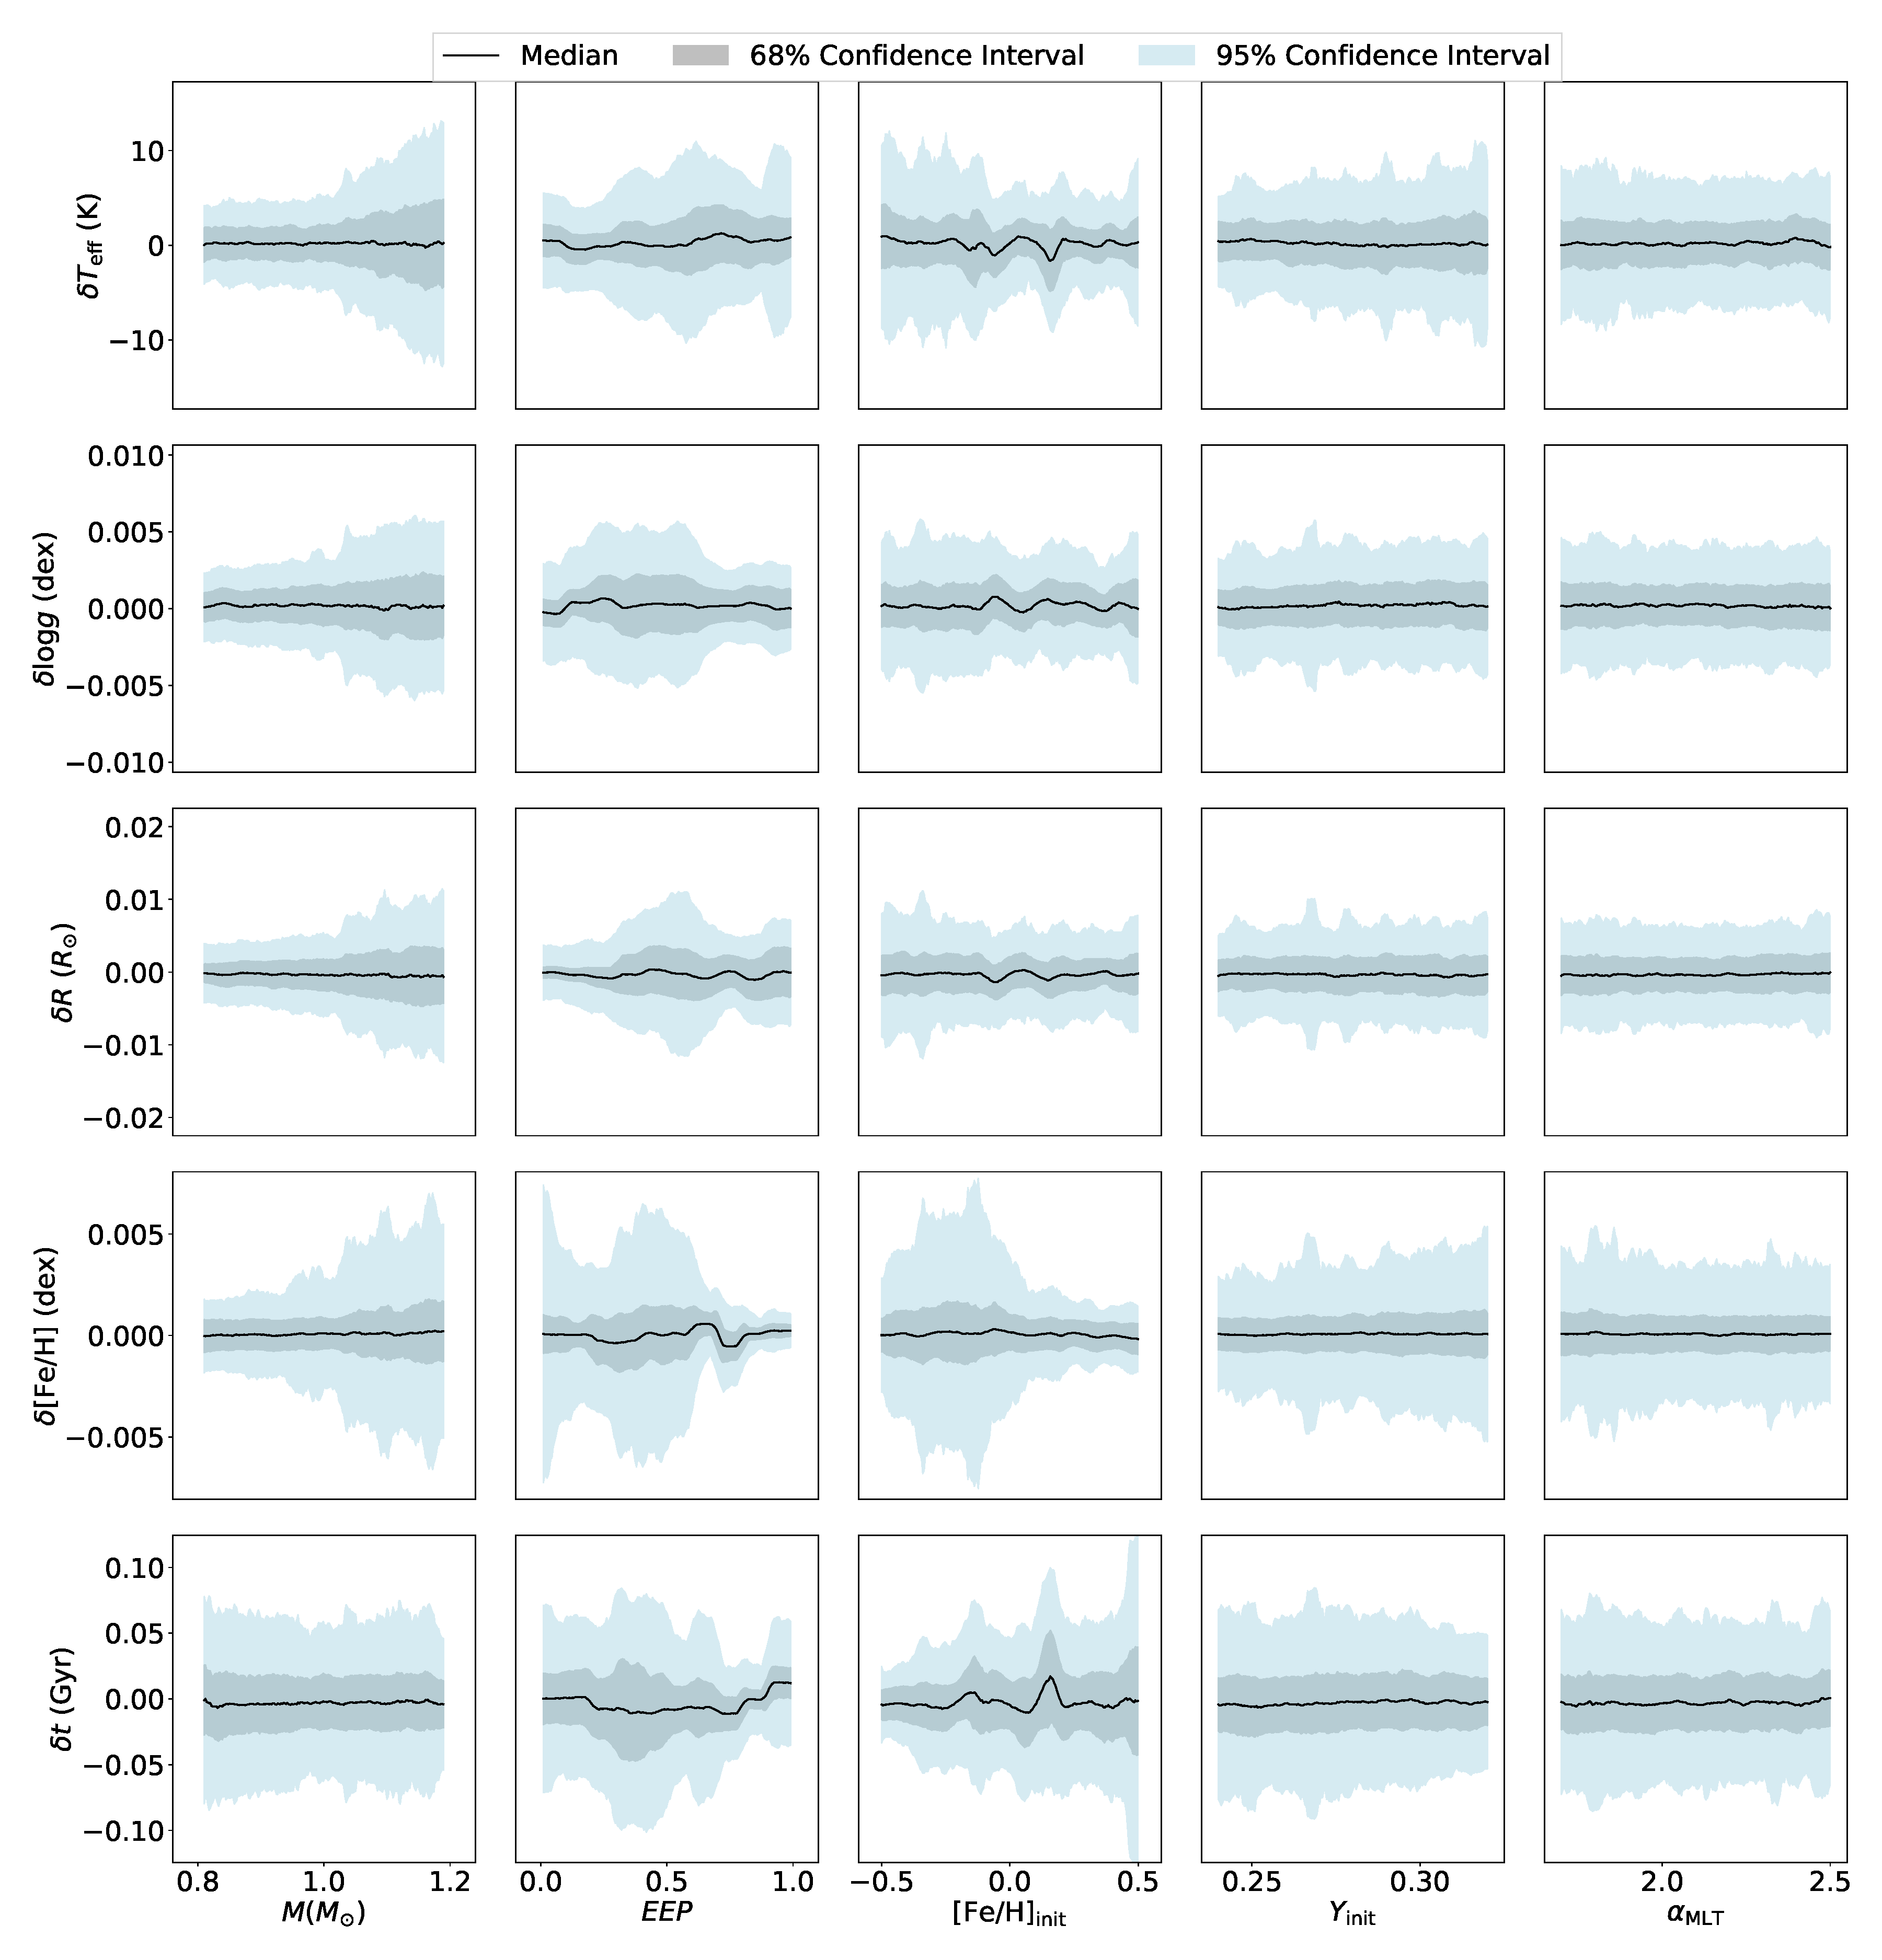
\includegraphics[width=2.0\columnwidth]{ 5d-testing_vs_inputs.pdf}
    \caption{ Roll medians and confidential interval of testing errors against GP model  inputs. Black solid line indicate the median; grey and blue shadow represent the 68\% and 95\% confidential interval. Testing errors of $T_{\rm eff}$, $\log g$, and $R$ mainly depend on $M$ and $EEP$. Metallicity error strongly depends on $M$, $EEP$, and [Fe/H]$_{\rm init}$, and age error has a significant correlation to $EEP$ and [Fe/H]$_{\rm init}$. However, testing errors do not obviously relate to $Y_{\rm init}$ or $\alpha_{\rm MLT}$. } 
  \label{fig:5d_test_vs_input}
\end{figure*}


\begin{itemize}
\item E vs output
\item E vs input 
\item E for on-grid and off-grid (validating and testing)
\item E on M-EEP diagram (optional)
\end{itemize}


\subsection{Systematical Uncertainties of GP Models}\label{sec:sys}



%\section{Modeling stars with GPR models}

%\subsubsection{Three Fake Stars}

%\subsubsection{The Sun}

%\subsubsection{Six {\em Kepler} Dwarfs and Subgiants}

\begin{itemize}
\item Accuracy goes down. Because the multiple-demission space size increase while the training dataset has a limitation of 10,000 points.  
\item We hence need to divide the grid into small chunks and train each chunk separately.  (illustrate how chunks are divided)
\item  show training and validation results in a fancy way. 
\end{itemize}











\section{Discussion and Conclusions (work with Guy)}\label{sec:conclusion}

In this work, we apply a machine-learning algorithm that involves a Gaussian process to augment a stellar grid. We train GP models for the stellar grid and obtain continuous functions that map fundamental inputs to observable outputs on a good accuracy level. We also train another set of GP models which describe the local systematic uncertainty of each output parameter. A GP-trained model set is then generated and we use it to model fake stars. The GP-based modelling is obviously advanced in modelling individual stars compared with the gird-based modelling because it provides continuous sampling. We lastly test GP-determined masses and ages by comparing them with true values and find good consistence. 

1. summary of what paper is done.
/what we did
/how it works
/consequence, we have better accuracy reflects the truth of uncertainty. 


2. Details of the GP/ comments on the application of GP: kernels, mean function/ training and prediction/uncertainty issue/how we fix that/

3. with the trained GP, we augment sparse grid. We fit stars. We get better age estimates, for other parameters, which are known to be sparse, can be properly characterised thank to the fully sampling. 

%\subsubsection*{Advantages}
%GP is a very efficient tool to augment a stellar grid instead of computing massive evolutionary tracks. For the case in this study, we train 10 GP-Grid models and 1 GP-SYS model for each output parameter and hence 55 GP models in total. The training process takes approximate one hour per GP model on a NVidia Tesla V100 graphics processing unit (GPU). 
%
%We also show that GP is able to manage the augmentation in high-demissions data (5 demissions in this work), which is very difficult for the interpolation approach.
%
%Moreover, the section scenario overcomes the limitation of training data size (20,000 for this case) and offers flexibility to apply GP on stellar grids with different size. 
%
%When modelling individual stars, GP significantly improves the sampling especially for initial metallicity, helium fraction, and the mixing-length parameter, which are always well spaced in a stellar grid. 
%

%{\bf Any more points?}    

%\subsubsection*{Limitations}
%GP is efficient for training global parameters but not for training the stellar structure. It hence not able to replace a stellar model. To obtain comprehensive stellar model, an optimal path would be using GP to constrain the range of fundamental parameters and then computing models with stellar code in that range.
%

%{\bf add more limitations}  

%\subsubsection*{Future works}

%This work presents an application of GP on augmenting the whole grid. However, this method is not efficient when modelling a single star. Our future work is developing a fast tool that only trains a small set of models in the grid around a star. This trained-GP model can be easily sticked with an Markov chain Monte Carlo simulator for a delicate bayesian analysis. 
%

%{\bf more future works} 

\section*{Acknowledgements}

Development of GPyTorch is supported by funding from the Bill and Melinda Gates Foundation, the National Science Foundation, and SAP.

%%%%%%%%%%%%%%%%%%%%%%%%%%%%%%%%%%%%%%%%%%%%%%%%%%

%%%%%%%%%%%%%%%%%%%% REFERENCES %%%%%%%%%%%%%%%%%%

% The best way to enter references is to use BibTeX:

\bibliographystyle{mnras}
\bibliography{ref} % if your bibtex file is called example.bib


%%%%%%%%%%%%%%%%%%%%%%%%%%%%%%%%%%%%%%%%%%%%%%%%%%

%%%%%%%%%%%%%%%%% APPENDICES %%%%%%%%%%%%%%%%%%%%%

%\appendix
%\onecolumn
%\appendix{}

\section{Setup of GP model training}\label{app:A}

This section includes detailed discussions about the selections of mean function, likelihood and loss function, optimiser, and early stopping. 

\subsection{Mean Function}

We first investigate the mean function. As discussed above, the data distribution is generally smooth but complex in some regions of parameter space (e.g., the sub-giant hook).  Although a GP model can cope with different mean functions,  because of the flexibility of kernels, we find that using a constant or a linear mean function leads to a long time for training. For this reason, we apply a Neural Network mean function which is flexible enough to manage both simple and complex features. We adopt an architecture including 6 hidden layers and 128 nodes per layer. All layers apply the linear transformation to the incoming data. We apply the element-wise function (Elu) because it give relatively smooth mean functions. ({\bf Can Guy or Alex add some references for NN and Elu here? The referee may ask why the 6x128 architecture is sufficient, so should we mention Alex's paper?})

\subsection{Likelihood and Loss Function}

Our training dataset is a theoretical model grid,  hence there is no observed uncertainty for each data point, but a tiny random uncertainty exists due to the approximations in the \textsc{MESA} numerical method. We model this using $\sigma_{w}$.  This noise model is then assumed to be a Gaussian function with a very small variance.  
%   
A likelihood specifies the mapping from input values $f(X)$ to observed labels $y$.
We adopt the the standard likelihood for regression which assumes a standard homoskedastic noise model whose conditional distribution is
\begin{equation}\label{eq:likelihood}
p(y|f(x)) = f + \epsilon, \epsilon \sim \mathcal{N}(0, \sigma^{2}),
\end{equation}
where $\sigma$ is a noise parameter. 
%
We used a small and fixed noise parameter and run a few tests.  However, the strict noise parameter makes GP models hard to converge. When this noise parameter is set as free, it reduces to a small value anyway in the training progress because it is data-driven.  For this reason, we did not put strict constraint for or prioritise this noise parameter.  In practice, we only set up a loose upper limit ($\sigma$  < 0.1) to speed up the training. One thing should be noted that a GP model with a large noise parameter is not a proper description for the stellar grid. Because of this, we only adopt GP models with $\sigma$ $\lesssim 10^{-4}$. We train GP models model using the negative logarithm of the likelihood function as the loss function.  

\subsection{Optimiser}

We compared two optimisers named SGD and Adam. Here SGD refers to Stochastic Gradient Descent, and Adam is a combination of the advantages of two other extensions of stochastic gradient descent, specifically, Adaptive Gradient Algorithm and Root Mean Square Propagation. 
%
The SGD optimiser in the \textsc{GPyTroch} package involves the formula given by \citet{sutskever2013importance}. The formula makes it possible to train using stochastic gradient descent with momentum thanks to a well-designed random initialisation and a particular type of slowly increasing schedule for the momentum parameter. The application of momentum in SGD could improve its efficiency and make it less likely to stuck in local minimums. On the other hand, the Adam optimiser includes the 'AMSGrad' variant developed by \citet{47409} to improve its weakness in the convergence to an optimal solution. With these new developments, the two optimisers give very similar results. We finally choose Adam because it works relatively efficiently and stable.  
%
We adaptive learning rate in the training process. Our training starts with a learning rate of 0.01 and decreases by a factor of 2 when the loss value does not reduce in previous 100 iterations.    

\subsection{Early Stopping}

We set up an Early Stopping for avoiding overfitting and also determining when to terminate a training progress. 
When an optimal solution is found, the validating errors stop decreasing and then increase when overfitting occurs. 
We hence track down the validating error every iteration and terminate training process when the validating error does not decrease in previous 300 iterations. 	

\section{State-of-the-art implement for large dataset}\label{app:B}

In section \ref{sec:3d}, we investigate the strategy for large dataset. We test two State-of-the-art approaches that designed for training big data whose data size is more than the limit of a GP model. Here we mention some details about the two methods and the results. 

We first consider the Stochastic Variational GP (SVGP) approach based on the \textsc{GPyTorch ApproximateGP} module. 
We train our data based on the SVGP example on \url{https://docs.gpytorch.ai/en/v1.1.1/examples/04_Variational_and_Approximate_GPs/SVGP_Regression_CUDA.html}. 
SVGP is an approximate scheme rely on the use of a series of inducing points which can be selected in the parameter space. It trains using mini batches and hence is able to deal with large data size. The other key point of SVGP is the number of inducing points. Because the kernel is only built on these points, the number determines the complexity of kernel. When the underline function is simple, for instance, a power law, a small number of inducing points  is enough. For our application, a large number of inducing points are required. Underline principles and detailed descriptions of this approach can be found in \citet{hensman2015scalable}. In our tests on 3D problem, we find a practical issue with the SVGP approach. When we load in a large training sample which takes a lot GPU memory, the rest memory can capacitate only 10,000 inducing points. This is to say, we use more training data but sacrifice the kernel complexity.  The result shows that using SVGP model does not improve the GP predictions compared with normal GP model. For instance, the 68th, 95th, and 99.7th testing errors for $T_{\rm eff}$ are 2.2, 6.8, and 15.1K (EI = 24.1 K) for the SVGP and 2.0, 5.8, and 15.7 K (EI = 23.5K) for the normal GP model. This is because the evolutionary feature are complex across multiple demissions. Reducing the kernel complexity is not ideal. We conclude that the SVGP is suitable for training large data which have relatively simple variations but not a good choice for training the model grid.  

We also investigate another approach designed for large dataset named Structured Kernel Interpolation (SKI GP). SKI GP was introduced by \citet{wilson2015kernel}. It produces kernel approximations for fast computations through kernel interpolation and is a great way to scale a GP up to very large datasets (100,000+ data points).
We follow the example on \url{https://docs.gpytorch.ai/en/stable/examples/02_Scalable_Exact_GPs/KISSGP_Regression.html} to develop our script. 
We run a few tests to train a 3D SKI GP model with 100, 000 training data. Compare with the Normal GP and SVGP, its testing errors for $T_{\rm eff}$ are slightly improved to 2.0, 6.1, and 14.8K (EI = 22.9K). However, the further test on the 5-demission data is not ideal: a SKI GP model using 100, 000 training data performs much worse than a normal model with only 20,000 training data. The poor behaviour consists with what has been discussed by \citet{wilson2015kernel}: the SKI GP poorly scale to data with high dimensions, since the cost of creating the grid grows exponentially in the amount of data. We attempt to make some additional approximations with the \textsc{GpyTorch AdditiveStructureKernel} module. It makes the base kernel to act as one-dimension kernels on each data dimension and the final kernel matrix will be a sum of these 1D kernel matrices. However, the testing errors are not significantly improved. 

%\begin{figure}
%	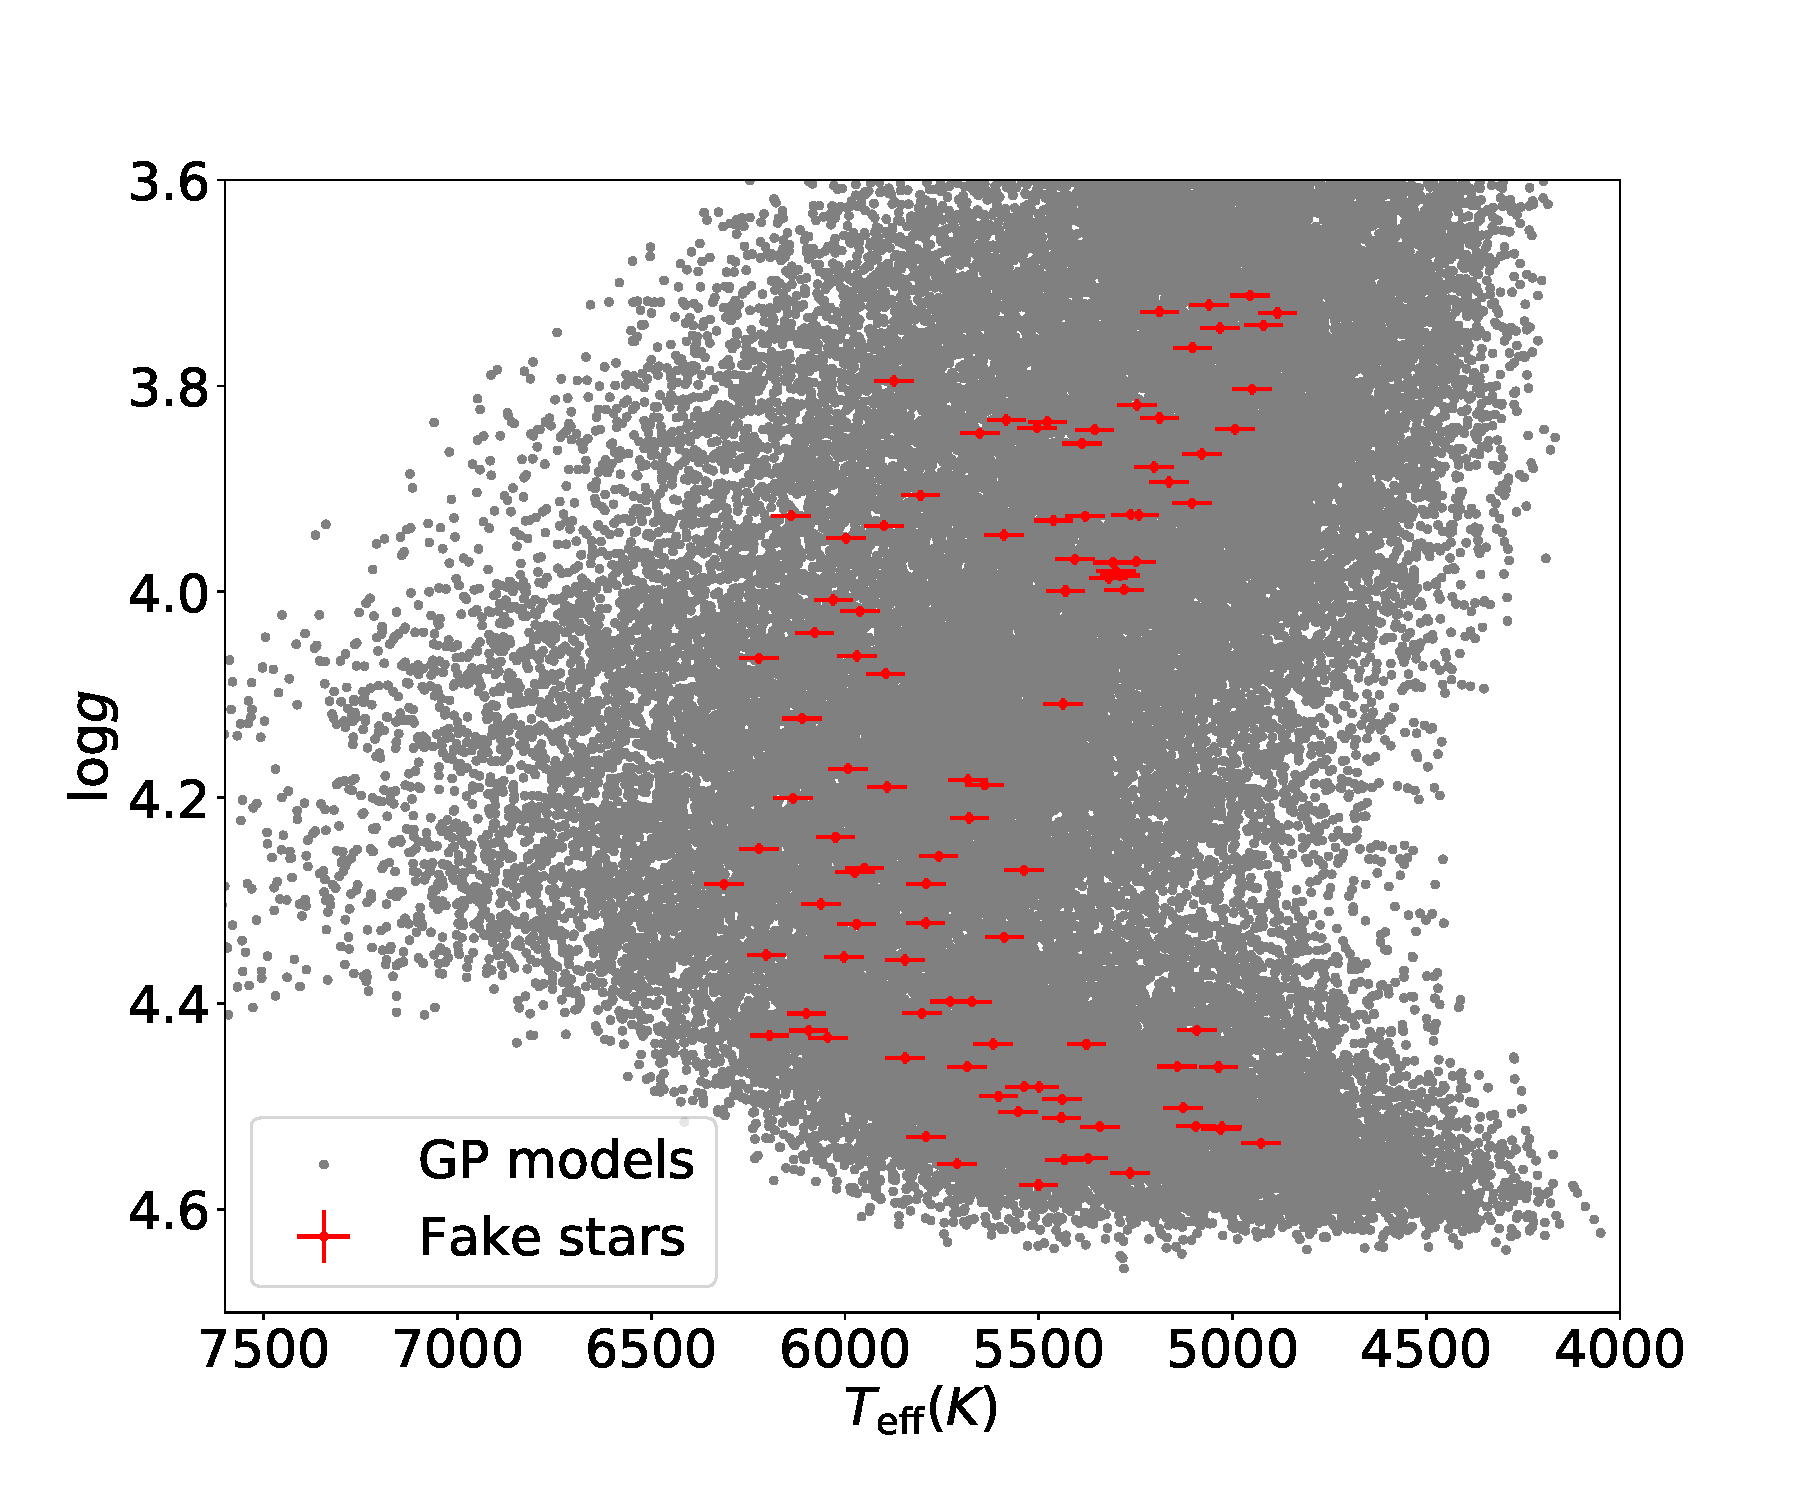
\includegraphics[width=1.0\columnwidth]{fake-stars-on-hrd.pdf}
%    \caption{Fake stars on the Keil diagram. } 
 % \label{fig:fit_comparison}
%\end{figure}






%%%%%%%%%%%%%%%%%%%%%%%%%%%%%%%%%%%%%%%%%%%%%%%%%%


% Don't change these lines
\bsp	% typesetting comment
\label{lastpage}
\end{document}

% End of mnras_template.tex